\documentclass[10pt,twocolumn,twoside]{IEEEtran}
% \def\BibTeX{{\rm B\kern-.05em{\sc i\kern-.025em b}\kern-.08em
%     T\kern-.1667em\lower.7ex\hbox{E}\kern-.125emX}}

\usepackage{amsmath}
\usepackage{bm}
\usepackage{nicefrac}
\usepackage{booktabs}
\usepackage{array}
\usepackage{multirow}
\usepackage{threeparttable}
\usepackage{makecell}
\usepackage[procnumbered,ruled,vlined,linesnumbered]{algorithm2e}
\usepackage{siunitx}
\usepackage{stfloats}
\usepackage{graphicx}
\usepackage{subfigure}
\usepackage{hyperref}
\usepackage{array}
\usepackage{epstopdf}
\usepackage{balance}
\usepackage{tabularx}
\usepackage{stfloats}
\usepackage{lipsum}

\newtheorem{problem}{Problem}
\newtheorem{theorem}{Theorem}[section]
\newtheorem{corollary}[theorem]{Corollary}
\newtheorem{lemma}[theorem]{Lemma}
\newtheorem{definition}[theorem]{Definition}
\newtheorem{fact}[theorem]{Fact}

% \newcommand{\proof}{{\bf Proof.}\hskip 0.3truecm}
% \newcommand{\endproof}{\quad \(\Box\)}

\newcommand{\defeq}{\stackrel{\mathrm{def}}{=}}
\newcommand{\setof}[1]{\left\{#1 \right\}}
% \newcommand{\sizeof}[1]{\left|#1 \right|}
\newcommand{\abs}[1]{\left|#1 \right|}
\newcommand{\mean}[1]{\mathbb{E}[#1]}
\newcommand{\ceil}[1]{\left\lceil#1\right\rceil}
\newcommand{\Abs}[1]{\left\Vert#1\right\Vert}
\newcommand{\trace}[1]{\mathrm{Tr}\left(#1\right)}

\newcommand{\bsym}[1]{\boldsymbol{#1}}
\newcommand{\myord}[1]{{#1}^{\rm{th}}}
\newcommand{\rea}{\mathbb{R}}
\newcommand{\gr}{\mathcal{G}}
\newcommand{\vecd}{\bsym{d}}
\newcommand{\veca}{\bsym{a}}
\newcommand{\vecb}{\bsym{b}}
\newcommand{\vece}{\bsym{e}}
\newcommand{\allone}{\bsym{1}}
\newcommand{\vecl}{\bsym{l}}
\newcommand{\vecv}{\bsym{v}}
\newcommand{\vecpi}{\bsym{\pi}}
\newcommand{\vecx}{\bsym{x}}

\newcommand{\pscr}{\mathscr{P}}

\newcommand{\lap}{\bsym{L}}
\newcommand{\matd}{\bsym{D}}
\newcommand{\mata}{\bsym{A}}
\newcommand{\matb}{\bsym{B}}
\newcommand{\matw}{\bsym{W}}
\newcommand{\matp}{\bsym{P}}
\newcommand{\matpcal}{\bsym{\mathcal{P}}}
\newcommand{\matf}{\bsym{F}}
\newcommand{\matfstar}{\bsym{F}^*}
\newcommand{\mati}{\bsym{I}}
\newcommand{\matq}{\bsym{Q}}
\newcommand{\matr}{\bsym{R}}
\newcommand{\mats}{\bsym{S}}
\newcommand{\matx}{\bsym{X}}
\newcommand{\maty}{\bsym{Y}}
\newcommand{\matz}{\bsym{Z}}
\newcommand{\matpi}{\bsym{\Pi}}

\newcommand{\lemref}[1]{Lemma~\ref{#1}}
\newcommand{\thmref}[1]{Theorem~\ref{#1}}
\newcommand{\probref}[1]{Problem~\ref{#1}}
\newcommand{\algoref}[1]{Algorithm~\ref{#1}}
\newcommand{\defref}[1]{Definition~\ref{#1}}
\newcommand{\secref}[1]{Section~\ref{#1}}
\newcommand{\tabref}[1]{Table~\ref{#1}}
\newcommand{\figref}[1]{Figure~\ref{#1}}

\newcommand{\edge}[2]{\langle #1, #2 \rangle}


\DeclareMathOperator*{\argmin}{arg\,min}
\DeclareMathOperator*{\argmax}{arg\,max}

\DontPrintSemicolon
\SetKw{KwAnd}{and}
\SetFuncSty{textsc}
\SetKwInOut{Input}{Input\ \ \ \ }

\SetKwInOut{Output}{Output}
\newcommand{\biophoto}[1]{\includegraphics[width=1in,height=1.25in,clip,keepaspectratio]{#1}}
\newcommand{\todo}[1]{{\bf \color{red} TODO: #1}}

\begin{document}

%\title{Absorbing Time of Random Walks\\ as a Node Group Centrality}
\title{Means of Hitting Times for Random Walks on Graphs: Connections, Computation, and Optimization}
\author{Haisong~Xia,
    Wanyue~Xu~\IEEEmembership{Student Member,~IEEE},
    Zuobai~Zhang,
    Zhuoqing~Song,
    Zhongzhi~Zhang~\IEEEmembership{Member,~IEEE}
    \thanks{This work was  supported  by the National Natural Science Foundation of China (No. U20B2051) and the Shanghai Municipal Science and Technology
        Major Project  (No. 2021SHZDZX03). Any correspondence should be addressed to Zhongzhi Zhang.
    }


    \thanks{
        Haisong Xia, Wanyue Xu and Zhongzhi Zhang are with the Shanghai Key Laboratory of Intelligent Information Processing, School of Computer Science, Fudan University, Shanghai 200433, China;
        Zhongzhi Zhang is also with the Shanghai Engineering Research Institute of Blockchain, Shanghai 200433, China. {\tt\small zhangzz@fudan.edu.cn}
    }
    \thanks{
        An earlier version of this paper was presented in part at the Thirteenth ACM International Conference on Web Search and Data Mining (WSDM)~\cite{ZhXuZh20} [DOI: 10.1145/3336191.3371777].
    }

}

\markboth{IEEE Transactions on Information Theory}
% {Xia \MakeLowercase{\textit{et al.}}: Absorbing Time of Random Walks as a Node Group Centrality}
{Xia \MakeLowercase{\textit{et al.}}: Means of Hitting Times for Random Walks on Graphs: Connections, Computation, and Optimization}

\IEEEtitleabstractindextext{
    \begin{abstract}
        For random walks on an undirected graph, the mean hitting time \(H_j\) from a vertex \(i\) chosen from the stationary distribution to the target vertex \(j\) can be used as a measure of importance for vertex \(j\), while the Kemeny constant \(K\) is the mean hitting time from a vertex \(i\) to a vertex \(j\) selected randomly according to the stationary distribution.
        Both quantities have found a large variety of applications in different areas.
        However, their high computational complexity limits their applications, especially for large networks with millions of vertices.
        In this paper, we first establish a connection between the two quantities, representing \(K\) in terms of \(H_j\) for all vertices.
        Subsequently, we extend the notion of mean hitting time to the case of multiple vertices, proposing a vertex group centrality called Group Walk Centrality (GWC).
        We then express these quantities in terms of either the pseudoinverse for graph Laplacian or the inverse for a SDDM matrix, based on which we develop an efficient algorithm that provides an approximation of \(H_j\) for all vertices and \(K\) in nearly linear time with respect to the edge number, with high probability.
        Moreover, we study the problem of finding a subset \(S\) of \(k\) vertices to minimize its GWC \(\manc{S}\), proving its NP-hardness.
        Based on the aforementioned algorithm, we provide another nearly linear greedy algorithm to solve the GWC minimization problem with a \(1-\frac{k}{k-1}\cdot\frac{1}{e}-\epsilon\) approximation factor for any error parameter \(\epsilon\in(0,1)\).
        Extensive experiment results on real-life and model networks validate both the efficiency and accuracy of our proposed algorithms.
    \end{abstract}

    \begin{IEEEkeywords}
        Random walk, hitting time, Kemeny constant, spectral algorithm, complex network, vertex centrality.
    \end{IEEEkeywords}
}

\maketitle

\IEEEdisplaynontitleabstractindextext

\IEEEpeerreviewmaketitle

\section{Introduction}\label{sec:intro}

\IEEEPARstart{A}{s} a powerful tool and method, random walks have found broad applications in various aspects.
Frequently cited examples include image segmentation~\cite{Le06}, random algorithm design~\cite{SaDi12}, collaborative recommendation~\cite{FoPiReSa07}, community detection~\cite{LaDeBa14}, among others.
A fundamental quantity related to random walks is hitting time~\cite{Lo93}, also called first-passage time~\cite{CoBeTeVoKl07}.
For a random walk on a graph, the hitting time \(H_{ij}\) from a vertex \(i\) to another vertex \(j\) is the expected time for the walker starting from \(i\) to visit \(j\) for the first time.
Hitting time is related to many problems and has been successfully applied to diverse areas, such as Hanoi problem with random move~\cite{WuZhCh11,QiDoZhZh20}, query suggestion~\cite{MeZhCh08}, and clustering algorithm~\cite{ChLiTa08}.

Except for the intrinsic interest of hitting time itself and its direct applications, many other relevant quantities related to random walks are encoded in or expressed in terms of this crucial quantity, for example, absorbing random-walk centrality~\cite{MaMaGi15} (or Markov centrality~\cite{WhSm03}), Kemeny constant~\cite{Hu14} and random detour time~\cite{BoRaZh11,RaZh13}.
As the name implies, the absorbing random-walk centrality is a measure for the importance of vertices on a graph.
For a vertex \(j\), its absorbing random-walk centrality \(H_j\) is defined by \(H_j=\sum_{i} \rho(i) H_{ij}\), where \(\rho(\cdot)\) is the starting probability distribution over all vertices.
Different from the shortest-path based centrality measures, random-walk based centrality metrics include the contributions from essentially all paths~\cite{Ne05}, and thus have a better discriminating power.

For random walks on a graph with \(n\) vertices, the Kemeny constant \(K\) is defined as the expected time for the walker starting from one vertex to second vertex selected randomly from the graph according to the stationary distribution \(\vecpi=\left(\pi_1, \pi_2, \cdots, \pi_n\right)^{\top}\) of the random walk, that is, \(K=\sum_{j} \pi_j H_{ij}\).
The Kemeny constant has also found a wealth of applications in different fields~\cite{Hu14}.
It can be utilized to gauge the efficiency of user navigation through the World Wide Web (WWW)~\cite{LeLo02}.
Moreover, the Kemeny constant is related to the mixing rate of an irreducible Markov chain~\cite{LePeWi09}, by regarding it as the expected time to mixing of the Markov chain~\cite{Hu06}.
Recently, the Kemeny constant has been applied to measure the efficiency of robotic surveillance in network environments~\cite{PaAgBu15} and to characterize the noise robustness of a class of protocols for formation control~\cite{JaOl19}.

\textbf{Motivations}. Despite the wide range of applications of the absorbing random-walk centrality and the Kemeny constant, it is a computational challenge to obtain their exact values.
By definition, both the absorbing random-walk centrality and the Kemeny constant are a partial average of some hitting times.
However, the exact value of hitting time between any pair of vertices in a graph involves all eigenvalues and eigenvectors of (normalized) Laplacian matrix associated with the graph~\cite{Lo93,LiZh13PRE}, the computation complexity of which is the cube of the vertex number.
Thus, for large realistic networks with millions of vertices, we cannot obtain their absorbing random-walk centrality and the Kemeny constant by resorting this straightforward method for computing hitting time. It is then of theoretical and practical interest to seek for alternative approximate approaches that scale to large networks.

%While computing absorbing random-walk centrality for a single vertex can be difficult, it is even more complex to find a group of \(k\) important vertices, which arises in many studies. For instance, in the field of wireless networks, sensor placement involves selecting an optimal subset of vertices to place sensors to sample physical signals~\cite{KrSiGu08,RaChVe14}, such as radiation or temperature. Another example is point cloud sampling~\cite{DiChWaBa20,ChTiFeVeKo17}, which requires selecting a representative subset of points to preserve the geometric features of reconstruction. Traditional methods of ranking individual vertices may not meet these requirements, making it necessary to propose a vertex group centrality.

Moreover, in various practical applications, many problems cannot be reduced to determining the importance of individual nodes, but are essentially to find a group of $k$ nodes that is the most important among all node groups, each containing exactly $k$ nodes. For example, how to place resources on a fixed number of $k$ peers in P2P networks, so that they are easily accessed by others~\cite{GkMiSa06}.  Again for instance, in the field of wireless networks, sensor placement involves selecting an optimal subset of vertices to place sensors to sample physical signals~\cite{KrSiGu08,RaChVe14}, such as radiation or temperature. Finally, in the context of point cloud sampling~\cite{DiChWaBa20,ChTiFeVeKo17}, it requires selecting a representative subset of points to preserve the geometric features of reconstruction. Recently, the absorbing random-walk centrality for an individual vertex~\cite{WhSm03} has been extended to a group of vertices~\cite{MaMaGi15}. Moreover, the problem of choosing \(k\) most important vertices was proposed, and an approximated algorithm was developed to solve the problem in cubic running time, which is not applicable to large networks. Thus, it is of great significance to propose a hitting time based centrality for vertex group and design fast algorithm to find the most important  $k$ vertices.


We introduce a new vertex group centrality called Group Walk Centrality (GWC) by extending absorbing random-walk centrality to the case of multiple vertices.
For a connected undirected graph and a vertex group \(S\), GWC \(\manc{S}\) is the expected hitting time for a random walker starting from a vertex \(u\) to an arbitrary vertex in \(S\). Here, vertex \(u\) is chosen based on the stationary distribution \(\vecpi\).
We also introduce the GWC minimization problem, which involves identifying the vertex group \(S^*\) with capacity \(k\) that minimizes GWC \(\manc{S^*}\).

For the absorbing random-walk centrality \(H_j=\sum_{i} \rho(i) H_{ij}\), we focus on the special case when the starting probability distribution \(\rho(\cdot)\) is the stationary distribution \(\vecpi=(\pi_1, \pi_2, \cdots, \pi_n)^{\top}\) of the random walk.
In other words, we study \(H_j=\sum_{i} \pi_i H_{ij}\), which has received considerable attention~\cite{TeBeVo09,Be09,Be16}.
We first express \(K\) in terms of \(H_j\) for all vertices, and further express \(H_j\) and \(K\) in terms of quadratic forms of pseudoinverse of the Laplacian matrix.

We then propose a fast algorithm called \textsc{ApproxHK} to compute approximate \(H_j\) for all vertices and \(K\) for the whole graph in nearly linear time of the number of edges, based on the Johnson-Lindenstrauss lemma~\cite{Ac01} and the Laplacian solver~\cite{SpTe04,Sp10,KoMiPe11,LiBr12,CoKyMiPaPeRaSu14,KySa16,GaKySp23}.

For Group Walk Centrality (GWC), we reformulate it as the inverse of a SDDM matrix.
Although the GWC minimization problem is proved to be NP-hard, we can utilize the monotonicity and supermodularity of GWC to develop a fast greedy algorithm called \textsc{ApproxMinGWC}.
\textsc{ApproxMinGWC} is based on \textsc{ApproxHK} and yields an approximation factor of \(1-\frac{k}{k-1}\cdot\frac{1}{e}-\epsilon\) for any error parameter \(\epsilon\in(0,1)\).

Finally, we experimentally demonstrate that our algorithms are accurate and are significantly faster than the direct exact computation of related quantities according to their definitions.

The primary version of our work has been published in WSDM '20: The Thirteenth ACM International Conference on Web Search and Data Mining~\cite{ZhXuZh20}. The contributions of the conference version are summarized as follows:

\begin{itemize}
    \item We express the absorbing random-walk centrality \(H_j\) and the Kemeny constant \(K\) in terms of quadratic forms of pseudoinverse of the Laplacian matrix.
    \item We propose an approximation algorithm called \textsc{ApproxHK} to compute \(H_j\) and \(K\) in nearly linear time of the number of graph edges.
    \item Numerical experiments reveal the accuracy and efficiency of \textsc{ApproxHK}.
\end{itemize}

In the conference version~\cite{ZhXuZh20}, we focus solely on the mean hitting time for a single vertex.
In the extended version, we broaden the concept of mean hitting time to encompass multiple vertices and introduce a vertex group centrality along with a corresponding minimization problem.
The following are our primary additional contributions:

\begin{itemize}
    \item We propose a vertex group centrality called Group Walk Centrality (GWC) based on the group hitting time.
    \item We introduce the GWC minimization problem, proving its NP-hardness.
    \item Due to the monotonicity and supermodularity of GWC, we develop an efficient greedy algorithm called \textsc{ApproxMinGWC} based on \textsc{ApproxHK} to approximately solve the GWC minimization problem.
    \item Extensive experiment results demonstrate that both of \textsc{ApproxHK} and \textsc{ApproxMinGWC} are accurate and scalable, which can be applied to networks with millions of vertices.
\end{itemize}


\section{Preliminaries}

In this section, we give a brief introduction to some notations, as well as some basic concepts about graphs, such as Laplacian matrix, resistance distance, random walks, hitting times, and some quantities derived from hitting times.

\subsection{Notations}

We use  \(\rea\) to deonte the set of real number, and we use normal lowercase letters such as \(a,b,c\) to represent scalars in \(\rea\). We denote vectors with bold lowercase letters such as \(\veca,\vecb,\vecc\), and matrices with bold uppercase letters like \(\mata,\matb,\matc\). For the convenience of representing specific elements in vectors and matrices, we use \(a_{i}\) to represent the \(\myord{i}\) element of vector \(\veca\), and use \(\mata_{[i,j]}\) to represent the entry at position \((i,j)\) in matrix \(\mata\). We use \(\mata_{[i,:]}\) and \(\mata_{[:,j]}\) to denote, respectively, the \(\myord{i}\) row and \(\myord{j}\) column of matrix \(\mata\). We write sets in subscripts to denote subvectors and submatrices.
For example, \(\mata_{[S,j]}\) represents the submatrix of \(\mata\), which includes those matrix elements with row indices in \(S\) and column index as \(j\). Similarly, \(\veca_{-S}\) represents the subvector of \(\veca\) obtained from  \(\veca\) by removing elements with indices in set \(S\), and \(\mata_{-S}\) represents the submatrix of \(\mata\) obtained  from  \(\veca\) by removing elements with row indices and column indices in set \(S\).
Note that the subscript takes precedence over the superscript, thus \(\mata_{-S}^{-1}\) denotes the inverse of \(\mata_{-S}\) rather than the submatrix of \(\mata^{-1}\). We use  \(\vecone_n\in \rea^n\) to denote a vector of \(n\) dimensions with all elements being \(1\). Sometimes we skip subscripts if there is no ambiguity. For a matrix \(\mata\in\rea^{m\times n}\), its Frobenius form is \(\Abs{\mata}_F=\sqrt{\trace{\mata^\top\mata}}\).

%We use \(\vece_i\) to denote the \(\myord{i}\) standard basis vector of particular dimensions, and use \(\vecone_n\in \rea^n\) to denote a vector of \(n\) dimensions with all elements being \(1\). Sometimes we skip subscripts if there is no ambiguity. For a matrix \(\mata\in\rea^{m\times n}\), its Frobenius form is \(\Abs{\mata}_F=\sqrt{\trace{\mata^\top\mata}}\).

%As we will prove the approximation guarantee of our algorithms in \secref{sec:approx-algo1} and \secref{sec:approx-algo2}, it is necessary to give the definition of approximation factor.


\begin{definition}[\(\epsilon\)-approximation]
    Let \(x\) and \(\tilde{x}\) be positive scalars, with \(\epsilon\) as the error parameter such that \(\epsilon\in(0,1)\). We refer to \(\tilde{x}\) as an \(\epsilon\)-approximation of \(x\) if the inequality \((1-\epsilon)x\le \tilde{x}\le(1+\epsilon)x\) holds. For convenience, we write this as \(x\approx_{\epsilon}\tilde{x}\).
\end{definition}



\subsection{Graph and Laplacian Matrix}\label{sub:lap}

Let \(\gr=(V,E,w)\) denote a connected undirected weighted graph or network,  where \(V\) is the set of vertices,  \(E\) is the set of edges, and  \(w: E\to \mathbb{R}_{+}\) is the positive edge weight function, with \(w_e\) being the weight for edge \(e\). Then, there are total \(n=\abs{V}\) vertices and \(m=|E|\) edges in graph \(\gr\). We use \(u \sim v\) to indicate that two vertices \(u\) and \(v\) are connected by an edge. Let \(w_{\max}\) and \(w_{\min}\) denote the maximum edge weight and minimum edge weight, respectively. Namely, \(w_{\max}=\max_{e\in E} w_e \) and \(w_{\min}=\min_{e\in E} w_e\).

Mathematically, the topological and weighted properties of a graph \(\gr\) are encoded in its generalized adjacency matrix \(\mata\) with the entry \(a_{ij}\) denoting the adjacency relation between vertices \(i\) and \(j\). If vertices \(i\) and \(j\) are linked to each other by an edge, then we denote this edge as \(e=\edge{i}{j}\), with \(a_{ij}= a_{ji}=w_{e}> 0\). If vertices \(i\) and \(j\) are not adjacent, \(a_{ij}=a_{ji}=0\). In a weighted graph \(\gr\), the degree \(d_i\) of a vertex \(i\) is defined by \(d_i=\sum_{j=1}^n a_{ij}\)~\cite{BaBaPaVe04}, where we denote the maximal vertex degree as \(d_{\max}=\max\setof{d_i|i\in V}\).
The diagonal degree vector of graph \(\gr\) is defined to be \(\vecd=\mypar{d_1,d_2,\cdots,d_n}^\top\), while the diagonal degree matrix of graph \(\gr\) is defined to be \({\matd} = {\rm diag}(d_1, d_2, \ldots, d_n)\), and the Laplacian matrix of \(\gr\) is \({\lap}={\matd}-{\mata}\). Thus, \(\lap\)  is a symmetric diagonally dominant (SDD) matrix. Moreover, for
any  nonempty  proper subset  \(S \) of vertex set $V$, \(\lap_{-S}\) is a symmetric diagonally dominant M-matrix (SDDM).

Let \(\matb \in \mathbb{R}^{|E| \times \abs{V}}\) be the incidence matrix of graph \(\gr\). For each edge \(e\) with two end vertices \(i\) and \(j\), a direction is assigned arbitrarily. Let \(\vecb_e^\top\) be the row of matrix \(\matb\) associated with edge \(e\). Then the element \(b_{eu}\) at row corresponding to edge \(e\) and column corresponding to vertex \(u\) is defined as follows: \(b_{eu} = 1\) if vertex \(u\) is the tail of edge \(e\), \(b_{eu}=-1\) if vertex \(u\) is the head of  edge \(e\), and \(b_{eu}=0\) otherwise. Let \(\vece_u\) be the \(u\)-th canonical basis of the space \(\mathbb{R}^{\abs{V}}\), then for an edge \(e\) connecting two vertices \(i\) and \(j\), \(\vecb_e\) can also be recast as \(\vecb_e=\vece_{i}-\vece_{j}\).  Let  \(\matw \in \mathbb{R}^{|E| \times |E|}\) be a diagonal matrix with every diagonal entry corresponding to the weight  \(w_e\) of an edge  $e\in E$. Then the Laplacian matrix \(\lap\) of graph \(\gr\) can be written as \(\lap=\matb^T\matw\matb=\sum_{e\in E}w_e\vecb_e\vecb_e^{\top}\).

The Laplacian matrix \(\lap\) is symmetric and positive semidefinite. All  its eigenvalues  are non-negative, with a unique zero eigenvalue. Let \(0=\lambda_1< \lambda_2 \leq \lambda_3\leq \dots\leq \lambda_{n}\) be the \(n\) eigenvalues of  \(\lap\), and let \(u_i\), \( i={1,2,\dots,n}\), be their corresponding mutually orthogonal  unit eigenvectors. Then, \(\lap\) has the following spectral decomposition:  \(\lap=\sum_{i=2}^{n}\lambda_i u_iu_i^\top\).  It is easy to verify that \( \lambda_{n}\leq n w_{\max}\)~\cite{LiSc18}.
Since \(\lap\) is not invertible, we use \(\lap^{\dagger}\) to denote its pseudoinverse, which can be written as \(\lap^{\dagger}=\sum_{i=2}^{n}\frac{1}{\lambda_i}u_iu_i^{\top}\). Let \(\matj\) denote the matrix with all entries being ones. Then the pseudoinverse \(\lap^{\dagger}\) can also be recast as \(\mypar{\lap +\frac{1}{n}\matj}^{-1} - \frac{1}{n}\matj\)~\cite{GhBoSa08}. Note that for a general symmetric matrix, it shares the same null space as its Moore-Penrose generalized inverse~\cite{BeGrTh74}.
Since the  null space of  null of \({\lap}\) is \( \vecone\),  it turns out that \({\lap} \vecone ={\lap}^{\dagger} \vecone =\mathbf{0}\). Note that for an invertible matrix, its pseudoinverse is exactly its inverse.

%Furthermore, the Laplacian matrix possesses several useful properties. It is easy to verify that Laplacian matrix is Symmetric Diagonally Dominant(SDD). Also, for a connected weighted undirected graph \(\gr=(V,E,w)\) and any nonempty vertex group \(S\), its corresponding Laplacian submatrix \(\lap_{-S}\) is Symmetric Diagonally Dominant M-matrix(SDDM).

\subsection{Electrical Network and Resistance Distance}

For an arbitrary graph \(\gr=(V,E,w)\), we can define its corresponding electrical network \(\bar{\gr}=(V,E,r)\), which is obtained from \(\gr\)  by considering edges as resistors and considering vertices as junctions between resistors~\cite{DoSn84}. The resistor of an associated  edge \(e\) is \(r_e=w_e^{-1}\).  For graph  \(\gr\), the resistance distance \(R_{ij}\) between two vertices \(i\) and \(j\)  is defined as the effective resistance between \(i\) and \(j\) in the corresponding  electrical network \(\bar{\gr}\)~\cite{KlRa93}, which is equal to the potential difference between \(i\) and \(j\) when a unit current enters one vertex and leaves the other one.

For graph \(\gr\), the resistance distance \(R_{ij}\) between two vertices \(i\) and \(j\) can be expressed in terms of the elements of \(\lap^{\dagger}\) as~\cite{KlRa93}:
\begin{equation}\label{EE04}
    R_{ij}={\lap}_{[i,i]}^{\dagger}+{\lap}_{[j,j]}^{\dagger}-2{\lap}_{[i,j]}^{\dagger}.
\end{equation}
Define \(\matr\) as the \(n \times n\) resistance matrix of graph \(\gr\), whose entry \(R_{[i,j]}\) at row \(i\) and column \(j\) represents the resistance distance \(R_{ij}\) between vertices \(i\) and \(j\).

\begin{lemma}\label{Foster} \cite{Te91}
    Let \(\gr=(V,E,w)\) be a simple connected graph with \(n\) vertices. Then the sum of  weight times resistance distance over all pairs of adjacent vertices in  \(\gr\)  satisfies
    \begin{equation*}
        \sum_{ i\sim j\in E }w_{ij}R_{ij}=n-1.
    \end{equation*}
    %where the summation is taken over all  edges in \(\gr\).
\end{lemma}

Similarly, We can also define the resistance distance \(R_{iS}\) between a vertex $i$ and a group  \(S\) of vertices. In the electrical network \(\bar{\gr}\) corresponding to graph \(\gr\), if all  the vertices in group \(S\) are grounded, the voltage of all vertices in set  \(S\) is always zero.
Then the resistance distance \(R_{iS}\) between vertex \(i\) and vertex group \(S\) is defined as the voltage of \(i\) when a unit current enters \(\bar{\gr}\) at vertex $i$ and leaves \(\bar{\gr}\) at  vertices in \(S\).  Let \(\pscr_{iS}\) denote a simple path connecting vertex \(i\) and an arbitrary vertex in \(S\). Then, the following relation holds:
\begin{equation}\label{eq:phy-resist}
    R_{iS}\le \sum_{\edge{a}{b}\in\pscr_{iS}}w_{ab}^{-1}\,.
\end{equation}

%Based on the physical explanation of effective resistance, the resistance distance \(R_{iS}\) is smaller than the effective resistance of any simple path connecting vertex \(i\) with any vertex \(j\in S To clarify, if we denote the simple path connecting vertex \(i\) and an arbitrary vertex in \(S\) as \(\pscr_{iS}\), then we have:


\subsection{Random Walk on a Graph}

For a connected weighted graph \(\gr\) with \(n\) vertices, the classical random walk on \(\gr\) can be described by the transition matrix \(\matp\in\rea^{n\times n}\). At any time step, the walker located at vertex \(i\) moves to vertex \(j\) with probability \({\matp_{[i,j]}=d_i^{-1}\mata_{[i,j]}}\).
It is easy to verify that
\begin{equation}\label{eq:trs}
    \matp=\matd^{-1}\mata.
\end{equation}

If  \(\gr\) is  finite and non-bipartite, the random walk  has a unique stationary distribution~\cite{LiZh13PRE}
\begin{equation}\label{EE01}
    \vecpi=(\pi_1, \pi_2, \cdots, \pi_n)^{\top}=\left(\frac{d_1}{d}, \frac{d_2}{d}, \cdots, \frac{d_n}{d}\right)^{\top},
\end{equation}
where \(d\) is the sum of degrees over all vertices, namely \(d=\sum_{i=1}^n d_i=\sum_{i=1}^{n}\sum_{j=1}^{n} a_{ij}\).

A fundamental quantity for random walks is hitting time~\cite{Lo93,CoBeTeVoKl07}. The hitting time \(H_{ij}\) from vertex \(i\) to vertex \(j\),  is the expected number of jumps for a walker starting  from \(i\) to visit \(j\) for the first time.
In other words, if we denote the time steps for a walker starting from \(i\) to first reach \(j\) as the random variable \(T_{ij}\), then we have \(H_{ij}=\mean{T_{ij}}\).
There is an intimate relationship between hitting time and resistance distance~\cite{Te91}.
\begin{lemma}
    Let \(\gr\) be a connected weighted graph with  resistance matrix  \(\matr\). Let \(H_{ij}\) be the hitting time  from vertex \(i\) to vertex \(j\). Then,
    \begin{equation}\label{EE03}
        H_{ij}=\frac{1}{2}\sum_{z=1}^{n} d_z(R_{ij}+R_{jz}-R_{iz}).
    \end{equation}
\end{lemma}

A lot of interesting quantities can be derived from hitting times. Here we only consider three quantities, the absorbing random-walk centrality~\cite{WhSm03,MaMaGi15}, the Kemeny constant~\cite{Hu14}, and the random detour time~\cite{BoRaZh11,RaZh13}.

For a vertex \(j\) in graph \(\gr=(V,E,w)\), its absorbing random-walk centrality \(H_j\) is defined as \(H_j=\sum_{i} \rho(i) H_{ij}\), where \(\rho(\cdot)\) is the starting probability distribution over all vertices in \(V\). By definition, \(H_j\) is a weighted average of hitting times to vertex \(j\). The smaller the value of \(H_j\), the more important the vertex \(j\). The random-walk based centrality has an obvious advantage over those shortest-path based centrality measures~\cite{Ne05}. In~\cite{WhSm03,MaMaGi15}, the uniform distribution for \(\rho(\cdot)\) is considered for the starting  vertices. In this paper, we concentrate on a natural choice of  \(\rho(\cdot)\) by selecting the starting vertex from the stationary distribution \(\vecpi\). In this case, \(H_j=\sum_{i} \pi_i H_{ij}\), which has been much studied~\cite{TeBeVo09,Be09,Be16}. In the following text, we  call \(H_j=\sum_{i} \pi_i H_{ij}\) \textit{walk centrality} for short.

Another quantity we are concerned with is the Kemeny constant \(K\). For a graph \(\gr\), its Kemeny constant \(K\) is defined as the expected steps for a walker starting from  vertex \(i\) to vertex \(j\) selected randomly from the vertex set \(V\), according to the stationary distribution \(\vecpi\). That is, \(K = \sum_{j = 1}^{n} \pi_j H_{ij}\). The Kemeny constant has been used to measure the user navigation efficiency through the WWW~\cite{LeLo02} and  robotic surveillance efficiency in network environments~\cite{PaAgBu15}. It can also measure the mixing rate of random walks~\cite{LePeWi09}.

%\textcolor{red}{Subsequently, for graph \(\gr\), its random detour time \(D_{ij}(u)\) is defined as the expected time of a walker who starts from vertex \(i\), must visit vertex \(u\), then first reaches vertex \(j\), where \(i,u,j\in V\) differs from each other. That is, \(D_{ij}(u)= H_{iu}+H_{uj}\).}

Most quantities for random walks on graph \(\gr\) are determined by the eigenvalues and eigenvectors of the normalized Laplacian matrix~\cite{Ch97}, \({\matd}^{-\frac{1}{2}}\lap {\matd}^{-\frac{1}{2}}\), of \(\gr\), including the walk centrality and Kemeny constant. By definition, \({\matd}^{-\frac{1}{2}}\lap {\matd}^{-\frac{1}{2}}\) is a real, symmetric, semi-definitive matrix. Let \(0=\sigma_1 < \sigma_2 \leq \sigma_3 \leq \cdots \leq \sigma_n \) be the \(n\) eigenvalues of the normalized Laplacian matrix \({\matd}^{-\frac{1}{2}}\lap {\matd}^{-\frac{1}{2}}\). And let \(\vecpsi_1\), \(\vecpsi_2\), \(\vecpsi_3\), \(\ldots\), \(\vecpsi_n\) be their corresponding mutually orthogonal eigenvectors of unit length, where \(\vecpsi_i=(\psi_{i1},\psi_{i2},\ldots,\psi_{in})^{\top}\). Then~\cite{Lo93,Be16},
\begin{equation}\label{ATT01}
    H_j=\sum_{i=1}^{n} \pi_i H_{ij}=\frac{d}{d_j}\sum_{k=2}^{n}\frac{1}{\sigma_{k}}\psi_{kj}^{2}
\end{equation}
and
\begin{equation}\label{Kemeny01}
    K =\sum_{j=1}^{n}\pi_j\,H_{ij} =\sum_{k=2}^{n}\frac{1}{\sigma_{k}}\,.
\end{equation}

Equations \eqref{ATT01} and \eqref{Kemeny01} provide exact computation for the walk centrality and Kemeny constant, respectively. However, both formulas are expressed in terms of the eigenvalues and eigenvectors of the normalized Laplacian, the computation complexity for which scale as \(O(n^3)\). Thus, direct  computation for \(H_j\) and \(K\)  using spectral method appears to be prohibitive for large networks, and is infeasible to those realistic networks with millions of vertices.

\section{Connections between Walk Centrality and  Kemeny Constant}

Although both the walk centrality \(H_j\) and the Kemeny constant \(K\) have attracted much attention from the scientific community, the relation between  them for a generic  graph  \(\gr\) is still lacking.
In this section, we establish an explicit relation between the walk centrality \(H_j\) and the Kemeny constant \(K\).
We then express both quantities in terms of quadratic forms of the pseudoinverse \(\lap^{\dagger}\) of graph Laplacian \(\lap\), which is helpful to address their computational challenges.

First, we show that the Kemeny constant \(K\) can be expressed in a linear combination of the walk centrality  \(H_j\) for all vertices in \(\gr\), as stated in the following lemma.
%Although both the walk centrality \(H_j\) and the Kemeny constant \(K\) have attracted much attention from the scientific community, the relation between  them for a generic  graph  \(\gr\) is still lacking. Below we show that the Kemeny constant \(K\) can be expressed in a linear combination of walk centrality  \(H_j\) for all vertices in \(\gr\), as stated in the following lemma.
\begin{lemma}
    Let \(\gr=(V,E,w)\) be a connected weighted graph. Then, its  Kemeny constant \(K\)  and walk centrality \(H_j\) obey the following relation:
    \begin{equation}\label{HjK01}
        K=\sum_{j=1}^{n} \pi_j H_j=\sum_{j=1}^{n} \frac{d_j}{d} H_j.
    \end{equation}
\end{lemma}
\begin{IEEEproof}
    From~\eqref{Kemeny01}, the Kemeny constant \(K\) is independent of the starting vertex \(i\). Define \(K_i =\sum_{j=1}^{n}\pi_j\,H_{ij}\). Then   \(K_i=K_j\) holds for any pair of vertices \(i\) and \(j\). Thus, we have
    \begin{align}\label{Kemeny02}
        K & =K_i =\sum_{i=1}^{n} \pi_i \left( \sum_{j=1}^{n}\pi_j\,H_{ij}\right) \notag \\
          & =\sum_{j=1}^{n} \pi_j \left( \sum_{i=1}^{n}\pi_i\,H_{ij}\right) \notag      \\
          & =\sum_{j=1}^{n} \frac{d_j}{d} H_j,\notag
    \end{align}
    which establishes the lemma.
\end{IEEEproof}

After obtaining the relation governing the Kemeny constant \(K\)  and walk centrality \(H_j\), we continue to express them in terms of quadratic forms of matrix  \(\lap^{\dagger}\).

\begin{lemma}\label{HjK}
    Let \(\gr=(V,E,w)\) be a connected weighted graph  with  Laplacian matrix \(\lap\). Then, the walk centrality \(H_j\) and Kemeny constant \(K\) can be represented  in terms of quadratic forms of the pseudoinverse \(\lap^{\dagger}\)  of   matrix  \(\lap\) as:
    \begin{equation}\label{ATT02}
        H_j=d(\vece_j - \vecpi)^{\top} \lap^{\dagger} (\vece_j - \vecpi)
    \end{equation}
    and
    \begin{equation}\label{Kemeny03}
        K= \sum_{j=1}^{n} d_j (\vece_j - \vecpi)^{\top} \lap^{\dagger} (\vece_j - \vecpi).
    \end{equation}
\end{lemma}
\begin{IEEEproof}
    We first prove~\eqref{ATT02}. Inserting~(\ref{EE03}) and~(\ref{EE04}) into~(\ref{ATT01}) leads to
    \begin{equation}\label{EE05}
        \begin{split}
            H_j&=\frac{1}{2} \sum_{i=1}^{n} \pi_i \sum_{z=1}^{n} d_z(R_{ij}+R_{jz}-R_{iz}) \\
            &=\frac{1}{d} \sum_{i=1}^{n} d_i \sum_{z=1}^{n} d_z \left({\lap}_{[j,j]}^{\dagger}-{\lap}_{[i,j]}^{\dagger}-{\lap}_{[j,z]}^{\dagger}+{\lap}_{[i,z]}^{\dagger}\right) \\
        \end{split}
    \end{equation}

    The four terms in the brackets of~\eqref{EE05} can be sequentially calculated as follows:
    \begin{equation}\label{EE06}
        \sum_{i=1}^{n} d_i \sum_{z=1}^{n} d_z {\lap}_{[j,j]}^{\dagger}=d^2 \vece_j^{\top} \lap^{\dagger} \vece_j\,,
    \end{equation}
    \begin{equation}\label{EE07}
        \sum_{i=1}^{n} d_i \sum_{z=1}^{n} d_z {\lap}_{[i,j]}^{\dagger}=\sum_{i=1}^{n} d_i \sum_{z=1}^{n} d_z {\lap}_{[j,z]}^{\dagger}=d^2 \vece_j^{\top} \lap^{\dagger} \vecpi\,,
    \end{equation}
    and
    \begin{equation}\label{EE08}
        \sum_{i=1}^{n} d_i  \sum_{z=1}^{n} d_z {\lap}_{[i,z]}^{\dagger}=d^2 \vecpi^{\top} \lap^{\dagger} \vecpi \,.
    \end{equation}
    Plugging~\eqref{EE06},~\eqref{EE07}, and~\eqref{EE08}  into~\eqref{EE05}, we obtain
    \begin{equation}\label{EE09}
        \begin{split}
            H_j&=d(\vece_j^{\top} \lap^{\dagger} \vece_j - 2 \vece_j^{\top} \lap^{\dagger} \vecpi + \vecpi^{\top} \lap^{\dagger} \vecpi) \\
            &=d(\vece_j - \vecpi)^{\top} \lap^{\dagger} (\vece_j - \vecpi).
        \end{split}
    \end{equation}
    Substituting~\eqref{EE09}  into~\eqref{HjK01} gives~\eqref{Kemeny03}.
\end{IEEEproof}

%According to \lemref{HjK}, we reduce the task of computing \(H_j\) and \(K\) to evaluating the quadratic forms of matrix \(\lap^{\dagger}\). Unfortunately,  direct computation of \(\lap^{\dagger}\) still has a complexity of \(O(n^3)\), which makes it impractical for larger networks.

%\section{Fast Approximation Algorithm for Computing \(H_j\) and \(K\)}

\section{Fast Approximation Algorithm for Walk Centrality and  Kemeny Constant}\label{sec:approx-algo1}

In the preceding section, we reduce the problem of computing  \(H_j\) and \(K\) to evaluating the quadratic forms \((\vece_u - \vecpi)^{\top} \lap^{\dagger} (\vece_u- \vecpi)\), \(u=1,2,\ldots, n\), of matrix  \(\lap^{\dagger}\).
However,  this involves computing the pseudoinverse of \(\lap\), the straightforward computation for which still has a complexity of \(O(n^3)\), making it infeasible to huge networks. Here, we present an algorithm to compute an approximation of \(H_u\) for all  \(u \in V\) and \(K\)  in nearly linear time with respect to the number of edges,  which has a strict theoretical guarantee with  high probability.

Let \(C(u)=(\vece_u - \vecpi)^{\top} \lap^{\dagger} (\vece_u- \vecpi)\), which can be written in an Euclidian norm as
\begin{small}
    \begin{equation}\label{EE12}
        \begin{split}
            C(u)&=(\vece_u - \vecpi)^{\top} \lap^{\dagger} \lap \lap^{\dagger} (\vece_u - \vecpi) \\
            &=(\vece_u - \vecpi)^{\top} \lap^{\dagger} \matb^{\top} \matw \matb \lap^{\dagger} (\vece_u - \vecpi) \\
            &=(\vece_u - \vecpi)^{\top} \lap^{\dagger} \matb^{\top} \matw^{\frac{1}{2}} \matw^{\frac{1}{2}} \matb \lap^{\dagger} (\vece_u - \vecpi) \\
            &=\|\matw^{\frac{1}{2}} \matb \lap^{\dagger} (\vece_u - \vecpi)\|^2.
        \end{split}
    \end{equation}
\end{small}
This  in fact  equals the square of the distance between  vectors  \(\matw^{\frac{1}{2}} \matb \lap^{\dagger} \vece_u\) and \(\matw^{\frac{1}{2}} \matb \lap^{\dagger} \vecpi\), which can be evaluated by the Johnson-Lindenstraus
Lemma (JL Lemma)~\cite{Ac01}.

\begin{lemma}[JL Lemma~\cite{Ac01}]
    \label{lemma:JL}
    Given $n$ fixed vectors \(\vecv_1,\vecv_2,\ldots,\vecv_n\in \mathbb{R}^d\) and
    \(\epsilon>0\), let
    \(\matq_{k\times d}\),  \(k\ge 24\log n/\epsilon^2\), be a matrix with each  entry equal  to \(1/\sqrt{k}\) or \(- 1/\sqrt{k}\)  with the same probability \(1/2\). Then with probability at least \(1-1/n\),
    \begin{equation*}
        \Abs{\vecv_i-\vecv_j}^2\approx_\epsilon\Abs{\matq\vecv_i-\matq\vecv_j}^2
    \end{equation*}
    for all all pairs  \(i,j\le n\).
\end{lemma}

\lemref{lemma:JL} indicates that,  the pairwise distances \(\|\vecv_i-\vecv_j\|^2\) (\(i,j=1,2,\ldots, n\)) are almost preserved if we project the \(n\) vectors \(\vecv_i\) (\(i=1,2,\ldots, n\))  into a lower-dimensional space, spanned
by \(O(\log n)\) random vectors.

In order to compute  \(C(u)\), we use Lemma~\ref{lemma:JL} to reduce the dimension. Let \(\matq\) be a \(k\times m\) random projection matrix. Then  \(\|\matq \matw^{\frac{1}{2}} \matb \lap^{\dagger}(\vece_u-\vecpi)\|\) is a good approximation for \(\|\matw^{\frac{1}{2}} \matb \lap^{\dagger} (\vece_u - \vecpi)\|\). Here we can use sparse matrix multiplication to compute \(\matq \matw^{\frac{1}{2}} \matb\). However, computing \(\matz=\matq \matw^{\frac{1}{2}} \matb \lap^{\dagger}\) directly involves inverting \(\lap+\frac{1}{n}\matj\). We avoid this by solving the system of equations \(\lap \vecz_i=\vecq_i\), \(i=1,\ldots,k\), where  \(\vecz^\top_i\) and \(\vecq^\top_i\) are, respectively, the \(i\)-th row of \(\matz\) and \(\matq \matw^{\frac{1}{2}} \matb\). For the convenience  of description, in the sequel we use the notation \(\Otil(\cdot)\) to hide \(\mathrm{poly} \log \) factors. By using Laplacian solvers~\cite{SpTe04,Sp10,KoMiPe11,LiBr12,CoKyMiPaPeRaSu14,KySa16}, \(\vecz^\top _i\) can be efficiently approximated.  We here use the  solver from~\cite{CoKyMiPaPeRaSu14}, the performance of which is characterized in \lemref{lemma:ST}.

\begin{lemma}[SDD Solver~\cite{CoKyMiPaPeRaSu14,KySa16,GaKySp23}]
    \label{lemma:ST}
    There is an algorithm \(\vecx = \mathtt{Solver}(\lap,\vecy,\delta)\) which
    takes a SDDM matrix or a Laplacian \(\lap\),
    a column vector \(\vecy\), and an error
    parameter \(\delta > 0\), and returns a column vector \(\vecx\) satisfying  \(\boldsymbol{1}^\top\vecx = 0\) and
    \[
        \|\vecx - \lap^{\dagger} \vecy\|_{\lap} \leq \delta \|\lap^{\dagger} \vecy\|_{\lap},
    \]
    where \(\Abs{\vecy}_{\lap} = \sqrt{\vecy^{\top} \lap \vecy}\).
    %The notation \(\lap^{\dagger}\) is used to represent the inverse matrix for a SDDM matrix or the pseudoinverse matrix for a Laplacian matrix.
    The algorithm runs in expected time \(\Otil \left(m \log(1/\delta) \right)\).
\end{lemma}

By Lemmas~\ref{lemma:JL} and~\ref{lemma:ST}, one can approximate \(C(u)\) arbitrarily well.

\begin{lemma}\label{lem:error1}
    Given an approximation factor \(\epsilon \le 1/2\) and a \(k\times n\) matrix \(\matz\) that satisfies
    \begin{equation*}
        C(u)\approx_\epsilon\Abs{\matz\mypar{\vece_u-\vecpi}}^2,
    \end{equation*}
    for any vertex \(u\in V\) and
    \begin{equation*}
        \Abs{\matw^{\frac{1}{2}}\matb\lap^\dagger\mypar{\vece_u-\vecv_v}}^2\approx_\epsilon\Abs{\matz\mypar{\vece_u-\vecv_v}}^2
    \end{equation*}
    for any pair of vertices \(u,v \in V\).
    Let \(\vecz_i\) be the \(i\)-th row of \(\matz\) and let \(\tilde{\vecz}_i\) be an approximation of \(\vecz_i\) for all \(i \in \{1,2,...,k\}\), satisfying
    \begin{equation}\label{EE13} \|\vecz_i-\tilde{\vecz}_i\|_{\lap}\le\delta
        \|\vecz_{i}\|_{\lap},
    \end{equation}
    where
    \begin{equation}\label{EE14}
        \delta \leq  \frac{\epsilon }{3} \frac{d-d_u}{d}
        \sqrt{\frac{(1-\epsilon) w_{\min}}{(1+\epsilon) n^4 w_{\max}}}.
    \end{equation}
    Then for any vertex \(u\) belonging to \(V\),
    %\begin{small}
    \begin{align}
        \label{EE15}
        (1 - \epsilon)^2  C(u)
        \leq
        \|\tilmatz  (\vece_{u} - \vecpi)\|^2
        \leq
        (1 + \epsilon)^2  C(u),
    \end{align}
    where \(\tilmatz = [\tilde{\vecz}_1, \tilde{\vecz}_2, ..., \tilde{\vecz}_k]^\top\).
    %\end{small}
\end{lemma}
\begin{IEEEproof}
    To prove (\ref{EE15}), it is sufficient  to show that for an arbitrary vertex \(u\),
    \begin{small}
        \begin{align}\label{EE16a}
             & \quad \abs{\Abs{\matz(\vece_u-\vecpi)}^2-\|{\tilmatz(\vece_u-\vecpi)}\|^2}\nonumber \\
             & =
            \abs{\Abs{\matz(\vece_u-\vecpi)}-\|\tilmatz(\vece_u-\vecpi)\|}\times \nonumber         \\
             & \quad\abs{\Abs{\matz(\vece_u-\vecpi)}+\|\tilmatz(\vece_u-\vecpi)\|} \nonumber       \\
             & \le
            \left(\frac{2\epsilon}{3}+\frac{\epsilon^2}{9}\right)\Abs{\matz(\vece_u-\vecpi)}^2,
        \end{align}
    \end{small}
    which is obeyed if
    \begin{small}
        \begin{equation}\label{EE16}
            \abs{\Abs{\matz(\vece_u-\vecpi)}-\|\tilmatz(\vece_u-\vecpi)\|} \le
            \frac{\epsilon}{3}\Abs{\matz(\vece_u-\vecpi)}.
        \end{equation}
    \end{small}
    This can be understood from the following arguments. On the one hand, if
    {\footnotesize \(\abs{\Abs{\matz(\vece_u-\vecpi)}^2-\|{\tilmatz(\vece_u-\vecpi)}\|^2} \le \left(\frac{2\epsilon}{3}+\frac{\epsilon^2}{9}\right)\Abs{\matz(\vece_u-\vecpi)}^2\)}, then
    \begin{align*}
            & \left(1-\frac{2\epsilon}{3}-\frac{\epsilon^2}{9}\right)\Abs{\matz(\vece_u-\vecpi)}^2  \\
        \le & \|{\tilmatz(\vece_u-\vecpi)}\|^2                                                      \\
        \le & \left(1+\frac{2\epsilon}{3}+\frac{\epsilon^2}{9}\right)\Abs{\matz(\vece_u-\vecpi)}^2,
    \end{align*}
    which, combining with \(\epsilon \le 1/2\) and the assumption that \(C(u)\approx_\epsilon\Abs{\matz\mypar{\vece_u-\vecpi}}^2\), leads to Eq.~\eqref{EE15}.
    On the other hand, if Eq.~\eqref{EE16} is true, we have \(\|\tilmatz(\vece_u-\vecpi)\| \le (1+\frac{\epsilon}{3})\Abs{\matz(\vece_u-\vecpi)}\). Thus,
    \begin{equation*}
        \abs{\Abs{\matz(\vece_u-\vecpi)}+\|\tilmatz(\vece_u-\vecpi)\|} \le (2+\frac{\epsilon}{3})\Abs{\matz(\vece_u-\vecpi)},
    \end{equation*}
    which results in Eq.~\eqref{EE16a}.

    We now prove that~\eqref{EE16} holds true.  By applying triangle inequality and Cauchy-Schwarz inequality, we obtain
    \begin{small}
        \begin{align*}
             & \quad \abs{\Abs{\matz(\vece_u-\vecpi)}-\|\tilmatz(\vece_u-\vecpi)\|}                                 \\
             & \le \Abs{(\matz-\tilmatz)(\vece_u-\vecpi)}                                                           \\
             & = \frac{1}{d} \Abs{\sum_{v=1}^{n} d_v (\matz-\tilmatz)(\vece_u-\vece_v)}                             \\
             & \le \frac{1}{d} \sum_{v=1}^{n} d_v \Abs{(\matz-\tilmatz)(\vece_u-\vece_v)}                           \\
             & \le \frac{1}{d} \sqrt{\sum_{v=1}^{n} d_v^2 \sum_{v=1}^{n} \Abs{(\matz-\tilmatz)(\vece_u-\vece_v)}^2} \\
             & \le \sqrt{\sum_{v=1}^{n} \Abs{(\matz-\tilmatz)(\vece_u-\vece_v)}^2},
        \end{align*}
    \end{small}
    where the last inequality is due to the fact that \(d=\sum_{v=1}^{n} d_v\ge \sqrt{\sum_{v=1}^{n} d_v^2}\).

    Since we only consider connected graphs,   there exists a simple path \(\mathcal{P}_v\) between \(u\) and any other vertex \(v\).  Applying the triangle inequality along path \(\mathcal{P}_v\), the square of the last sum term in the above equation can be evaluated as:
    \begin{small}
        \begin{align*}
             & \quad \sum_{v=1}^{n} \Abs{(\matz-\tilmatz)(\vece_u-\vece_v)}^2                                             \\
             & \le \sum_{v=1}^{n} \left(\sum_{a\sim b \in \mathcal{P}_v} \Abs{(\matz-\tilmatz)(\vece_a-\vece_b)}\right)^2 \\
             & \le n \sum_{v=1}^{n} \sum_{a\sim b \in \mathcal{P}_v} \Abs{(\matz-\tilmatz)(\vece_a-\vece_b)}^2            \\
             & \le n^2 \sum_{a\sim b \in E} \Abs{(\matz-\tilmatz)(\vece_a-\vece_b)}^2                                     \\
             & = n^2 \Abs{(\matz - \tilmatz ) \matb^{\top}}_{F}^{2}                                                       \\
             & = n^2 \Abs{\matb(\matz - \tilmatz )^{\top}}_{F}^{2}                                                        \\
             & \leq
            \frac{n^2}{w_{\min}} \Abs{\matw^{1/2} \matb(\matz - \tilmatz )^{\top}}_{F}^{2}\,.
        \end{align*}
    \end{small}
    % where \(\| \matm \|_{F}\) denotes the Frobenius norm of  matrix \(\matm\),  defined as the square root of the trace for matrix \(\matm^{\top} \matm\). 
    The last term can be bounded as
    \begin{small}
        \begin{align*}
                & \frac{n^2}{w_{\min}} \Abs{\matw^{1/2} \matb(\matz - \tilmatz )^{\top}}_{F}^{2}                      \\
            =   & \frac{n^2}{w_{\min}} \trace{(\matz - \tilmatz )\matb^{\top} \matw \matb(\matz - \tilmatz )^{\top}}  \\
            =   & \frac{n^2}{w_{\min}} \trace{(\matz - \tilmatz )\lap(\matz - \tilmatz )^{\top}}                      \\
            =   & \frac{n^2}{w_{\min}} \sum_{i=1}^k (\vecz_i - \tilde{\vecz}_i)^\top \lap (\vecz_i - \tilde{\vecz}_i) \\
            \le & \frac{n^2\delta^2}{w_{\min}} \sum_{i=1}^k \vecz_i^\top\lap\vecz_i                                   \\
            =   & \frac{n^2\delta^2}{w_{\min}}  \trace{\matz\lap\matz^{\top}}                                         \\
            =   & \frac{n^2\delta^{2}}{w_{\min}} \Abs{\matw^{1/2} \matb \matz^{\top}}_{F}^{2}\,,
        \end{align*}
    \end{small}
    where the  inequality follows from (\ref{EE13}) and the last term can be further evaluated by Lemma~\ref {Foster} as
    %\begin{small}
    \begin{align*}
         & \quad \frac{n^2\delta^2}{w_{\min}} \Abs{\matw^{1/2} \matb \matz^{\top}}_{F}^{2}                                            \\
         & =\frac{n^2\delta^{2}}{w_{\min}}
        \sum_{a\sim b \in E} w_{a\sim b} \Abs{\matz (\vece_{a} - \vece_{b})}^{2}                                                      \\
         & \leq
        \frac{\delta^{2}n^2 (1+\epsilon)}{w_{\min}}
        \sum_{a\sim b \in E} w_{a\sim b}\|\matw^{\frac{1}{2}} \matb \lap^{\dagger} (\vece_a-\vece_b)\|^2                              \\
         & =
        \frac{\delta^{2}n^2 (1+\epsilon)}{w_{\min}}
        \sum_{a\sim b \in E} w_{a\sim b}(\vece_a-\vece_b)^\top \lap^{\dagger} \matb^\top \matw \matb \lap^{\dagger} (\vece_a-\vece_b) \\
         & =
        \frac{\delta^{2}n^2 (1+\epsilon)}{w_{\min}}
        \sum_{a\sim b \in E} w_{a\sim b}(\vece_a-\vece_b)^\top \lap^{\dagger} \lap \lap^{\dagger} (\vece_a-\vece_b)                   \\
         & =
        \frac{\delta^{2}n^2 (1+\epsilon)}{w_{\min}}
        \sum_{a\sim b \in E} w_{a\sim b}(\vece_a-\vece_b)^\top \lap^{\dagger} (\vece_a-\vece_b)                                       \\
         & =
        \frac{\delta^{2} n^2 (1+\epsilon)}{w_{\min}}
        \sum_{a\sim b \in E} w_{a\sim b} R_{ab}                                                                                       \\
         & =\frac{\delta^{2} n^2(n-1) (1+\epsilon)}{w_{\min}},
    \end{align*}
    %\end{small}
    where $w_{a\sim b}$ represents the weight of the edge with endvertices $a$ and $b$.
    %The last inequality follows by the fact that  \(\sum_{a\sim b \in E} w_{a\sim b} R_{ab} = n-1\).

    In addition, \(\Abs{\matz (\vece_u - \vecpi)}^2\) can also be bounded by
    \begin{equation}\label{EE17}
        \begin{split}  \notag
            &\quad\Abs{\matz (\vece_u - \vecpi)}^2
            \geq
            (1 - \epsilon) C(u) \\
            &=(1-\epsilon)(\vece_u-\vecpi)^{\top} \lap^{\dagger} (\vece_u-\vecpi) \\
            &\geq (1-\epsilon)\lambda_{n}^{-1} \Abs{\vece_u-\vecpi}^2 \\
            &	\geq (1-\epsilon)(n w_{\max})^{-1} \frac{(d-d_u)^2}{d^2}.
        \end{split}
    \end{equation}
    In the above equation, the first inequation follows due to the following reason.   Note that \(\vece_u-\vecpi\) is orthogonal to  vector \(\vecone\), which is an eigenvector of \(\lap^{\dagger}\) corresponding to the \(0\) eigenvalue. Hence, \((\vece_u-\vecpi)^{\top} \lap^{\dagger} (\vece_u-\vecpi) \ge \lambda_{n}^{-1} \Abs{\vece_u-\vecpi}^2\) always holds true.

    %where \(\lambda_n\) refers to the maximum eigenvalue of \(L\). The last inequality in (\ref{EE17}) is due to the fact that \(w_{\max}\lap_{\mathcal{K}_n}-\lap_{G}\) is positive semidefinite, while \(\lap_{\mathcal{K}_n}\) is the Laplacian of an \(n\)-vertex clique whose edge weights are all equal to \(1\).
    Thus, we have
    %\begin{small}
    \begin{align*}
         & \quad \frac{
            \abs{ \Abs{\matz (\vece_{u} - \vecpi)} -  \Abs{\tilmatz  (\vece_{u} - \vecpi)}}
        }{
            \Abs{\matz (\vece_{u} - \vecpi)}
        }                                                 \\
         & \le
        \delta \left(\frac{n^2(n-1) (1+\epsilon)}{w_{\min}}\right)^{1/2}\left(\frac{n
        w_{\max}}{1-\epsilon}\right)^{1/2}\frac{d}{d-d_u} \\
         & \le \frac{\epsilon}{3},
    \end{align*}
    %\end{small}
    where \(\delta\) is given by (\ref{EE14}).
\end{IEEEproof}

Lemma~\ref{lem:error1} leads to the following theorem.
\begin{theorem}
    \label{TheoAlg1}
    There is a \(\Otil(m\log{c}/\epsilon^2)\) time algorithm, which  inputs  a scalar \(0<\epsilon<1\) and a graph \(\gr=(V,E,w)\) where \(c=\frac{w_{\max}}{w_{\min}}\), and returns a \((24\log n/\epsilon^2)\times n\) matrix \(\tilmatz\) such that with probability at least \(1-1/n\),
    \begin{align}
        (1-\epsilon)^2  C(u) \leq \|\tilmatz(\vece_u-\vecpi)\|^2 \leq (1+\epsilon)^2  C(u)\nonumber
    \end{align}
    for any vertex \(u \in V\).
\end{theorem}

Based on Theorem~\ref{TheoAlg1}, we  present an algorithm \textsc{ApproxHK} to approximately compute the walk centrality \(H_u\) for all  vertices  \(u \in V\) and the Kemeny constant \(K\), the pseudocode of which is provided in Algorithm~\ref{ALG01}.

\begin{algorithm}
    \caption{\textsc{ApproxHK}\((\gr, \epsilon)\)}
    \label{ALG01}
    \Input{
        \(\gr\): a connected undirected graph. \\
        \(\epsilon\): an approximation parameter %of vertex centrality
    }
    \Output{
        \(\tilde{H}=\{u,\tilde{H}_u| u \in V\}\): \(\tilde{H}_u\) is an approximation of the walk centrality \(H_u\) of vertex \(u\);
        \(\tilde{K}\): approximation of the Kemeny constant \(K\)
    }
    \(\lap=\) Laplacian of \(\gr\),\, \(d_u=\) the degree of \(u\) for all \(u\in V\), \(d=\sum_{u \in V} d_u\)\;  Construct a matrix \(\matq_{k \times m}\),  where \(k=\lceil 24\log n/\epsilon^2 \rceil\) and each entry is \(\pm 1/\sqrt{k}\) with identical probability\;
    \For{\(i=1\) to \(k\)}{
        \(\vecq_i^\top \)=the \(i\)-th row of  \(\matq_{k \times m} \matw^{1/2} \matb\)  \\
        \(\tilde{\vecz}_i=\mathtt{Solver}(\lap, \vecq_i, \delta)\) where parameter   \(\delta\) is  given by~(\ref{EE14}) \\
    }
    Calculate the constant vector \({\bf p}=\tilmatz \vecpi\)\;
    \For{each \(u\in V\)}{
    \(\tilde{H}_u=d \|\tilmatz_{:,u}-{\bf p}\|^2\)
    }
    \(\tilde{K}=\sum_{u \in V} \frac{d_u}{d} \tilde{H}_u\)\;
    \Return \(\tilde{H}=\{u,\tilde{H}_u| u \in V\}\) and \(\tilde{K}\)
\end{algorithm}

\section{Group Walk Centrality}

In this section, we extend the walk centrality \(H_j\) to the case of a group  $S$ of  vertices, denoted as \(H(S)\) and called Group Walk Centrality (GWC), which measures the relative importance of the vertex group $S$. We first give the definition of GWC. Then, we provide an examination of GWC, by establishing a connection between GWC and random detour time and the Kemeny constant. Finally, we show that as a set function \(\manc{\cdot}\), GWC is monotonic and supermodular.

%After presenting the walk centrality \(H_j\) and the Kemeny constant \(K\), we extend the notion of mean hitting time to the case of multiple vertices. In this section, we provide the definition of Group Walk Centrality (GWC). We also discuss the connections between GWC and other quantities related to random walk, such as the random detour time, the Kemeny constant and the equivalent electrical network of the augmented graph. Furthermore, we demonstrate monotonicity and supermodularity of GWC \(\manc{\cdot}\).

\subsection{Definition and Expression}

We utilize absorbing random walks with multiple traps~\cite{ZhYaLi12} to define GWC. For random walks on a connected graph \(\gr=(V,E)\) with vertices in set  \(S\) being traps (absorbing vertices), the hitting time (absorbing time) \(H_{iS}\) from vertex \(i\) to vertex group \(S\) is the expected number of steps for a walker starting from \(i\) to visit any vertex of \(S\) for the first time. If we denote the time steps for a walker starting from \(i\) to first reach an arbitrary vertex in \(S\) as random variable \(T_{iS}\), then we have \(H_{iS}=\mean{T_{iS}}\). Based on the hitting time \(H_{iS}\) to a vertex group $S$, we define the GWC of a set of vertices.


\begin{definition}[Group Walk Centrality, GWC]\label{def:manc}
    For a given vertex group \(S\) in a connected undirected graph \(\gr=(V,E)\), its GWC \(\manc{S}\) is defined as the expected time for a random walker starting from a vertex chosen from \(\gr\) according to the stationary distribution \(\vecpi\), to reach any vertex in \(S\).  Mathematically, \(\manc{S}\) is expressed as follows:
    \begin{equation*}
        \manc{S}=\sum_{i\in V}\pi_i H_{iS}.
    \end{equation*}
\end{definition}
Note that for the case that set \(S\) contains only one vertex \(j\), GWC \(\manc{S}\) reduces to walk centrality \(H_j\). If  \(\manc{S}\) is larger, then the vertices in  \(S\) are not easily accessible, which means that the vertices in  \(S\) are more peripheral, and are thus less important;  if  \(\manc{S}\) is smaller, then the vertices in  \(S\) are more important.

We now give an expression for \(\manc{S}\). For random walks in graph \(\gr=(V,E)\) with absorbing vertex group \(S\) and transition matrix \(\matp\),  the fundamental matrix \(\matf\) is~\cite{ZhYaLi12}    \begin{equation}\label{eq:funda}
    \matf=\sum_{l=0}^\infty\matp_{-S}^l=(\mati-\matp_{-S})^{-1}=(\mati-\matp)_{-S}^{-1}.
\end{equation}
From~\eqref{eq:funda}, we can see that  the entry \(\matf_{[i,j]}\) of matrix  \(\matf\) is the expected number of times a random walker starting from vertex \(i\) visits vertex \(j\) before being absorbed by vertices in  \(\manc{S}\). Then, \(\manc{S}\)  can be expressed as
\begin{equation*}
    \manc{S}=\vecpi_{-S}^\top\matf\vecone=\vecpi_{-S}^\top(\mati-\matp)_{-S}^{-1}\vecone.
\end{equation*}
By using~\eqref{eq:trs}, \(\manc{S}\) can be further written as
\begin{equation}\label{eq:GWC}
    \begin{split}
        \manc{S} & =\vecpi_{-S}^\top\mypar{\mati-\matd^{-1}\mata}_{-S}^{-1}\vecone                          \\
        & =\vecpi_{-S}^\top\mypar{\mati-\matd^{-1}\mata}_{-S}^{-1}\matd_{-S}^{-1}\matd_{-S}\vecone \\
        & =\vecpi_{-S}^\top\lap_{-S}^{-1}\vecd_{-S}.
    \end{split}
\end{equation}
Since $\lap_{-S}$ is an SDDM matrix, according to~\eqref{eq:GWC} and \lemref{lemma:ST}, we can approximately compute GWC of any given vertex group \(S\) by calling \(\mathtt{Solver}\mypar{\lap_{-S},\vecd_{-S},\delta}\). We omit the detail of this approximation algorithm, since  it simply utilizes~\lemref{lemma:ST}.


%Based on~\eqref{eq:funda}, we can express \(\matf_{[i,j]}\) as the expected number of times a random walker passes through vertex \(j\) before being absorbed, starting from vertex \(i\). According to the linearity of the mean, the hitting time of a random walker is equivalent to the sum of the expected number of passages through all vertices in the graph. That is, if we let \(l_i\) denote the hitting time of a random walker starting from vertex \(i\), then \(\vecl=\matf\vecone\). In particular, if the random walker starts from an absorbing vertex, the hitting time can be considered as zero. Considering the aforementioned case, we can express GWC \(\manc{S}\) as






%\subsection{Two Explanations }

\subsection{Connection with Other Quantities of Random Walks}

%In this subsection, we provide two explanations for GWC \(\manc{S}\) in graph \(\gr=(V,E)\). First, we establish a link between GWC $H(S)$ and some other quantities related to hitting times for  random walks without traps in \(\gr=(V,E)\). Then, we provide interpretation for  \(\manc{S}\)  in terms of voltages of an electrical network corresponding to augmented graph of \(\gr=(V,E)\).

%Here we establish a connection between GWC \(\manc{S}\) and some other quantities about hitting times. 


In this subsection, we establish a link between GWC $H(S)$  in graph \(\gr\) and some other quantities related to hitting times for random walks without traps in \(\gr\).

We first introduce a notion of random detour walk $i\rightarrow S \rightarrow j$. It is a random walk starting from a vertex $i$, that must visit at least a vertex in set $S$ before it arrives at the target vertex $j$ and stops. The group random detour time  \(D_{ij}(S)\) for the random detour walk $i\rightarrow S \rightarrow j$ is defined as the expected time for the walker starting from vertex \(i\) to visit at least a vertex in group \(S\), and then reaches vertex \(j\) for the first time. Note that when set $S$ includes only one vertex $k$, $i\rightarrow S \rightarrow j$ and \(D_{ij}(S)\) are reduced to the corresponding notion and quantity previously proposed in~\cite{RaZh13,BoRaZh11} for a single vertex.


For an absorbing random walks in graph \(\gr=(V,E)\)  with vertices in set \(S\)  being absorbing ones,  we denote the probability that a walker starting from vertex \(i\) first reaches vertex \(u\) in absorbing group \(S\) as the \(\myord{(i,u)}\) entry of matrix \(\matpdistr\in\rea^{n\times\abs{S}}\). Then, \(D_{ij}(S)\) can be expressed as
\begin{equation}
    D_{ij}(S)= H_{iS}+\sum_{k=1}^{\abs{S}}\matpdistr_{[i,k]}H_{kj}.
\end{equation}
This expression shows that  if \(D_{ij}(S)\) is larger, then it is difficult for a walker to reach vertices in \(S\), which indicates that vertices in \(S\) are relatively less significant in the overall network. Thus, \(D_{ij}(S)\) is consistent with the quantity $H_{iS}$. This enlightens us to explore the relation between \(\manc{S}\) and related quantities about hitting times, such as  \(D_{ij}(S)\). Theorem~\ref{thm:connection-multiple} establishes a link governing GWC \(\manc{S}\), group random detour time \(D_{ij}(S)\), and the Kemeny constant \(K\).


\begin{theorem}\label{thm:connection-multiple}
    For an arbitary vertex group \(S\subseteq V\) in a connected graph \(\gr=(V,E)\) with \(n\) vertices,
    \begin{equation}\label{eq:connection-multiple}
        \manc{S}+K=\sum_{i=1}^n\sum_{j=1}^n\pi_i\pi_jD_{ij}(S).
    \end{equation}
\end{theorem}
\begin{IEEEproof}
    To prove~\eqref{eq:connection-multiple}, we first introduce the fundamental matrix \(\matfstar\) for the non-absorbing random walk model on graph  \(\gr=(V,E)\).
    According to the results in~\cite{BoRaZh11}, \(\matfstar\) can be represented as \(\matfstar=(\mati-\matp+\vecone\vecpi^\top)^{-1}\matpi^{-1}\), where \(\matpi\) is defined as \(\rm{diag}\mypar{\vecpi}\).
    Then, the hitting time \(H_{ij}\) can be represented in terms of the elements of matrix \(\matfstar\) as \(H_{ij}=\matfstar_{[j,j]}-\matfstar_{[i,j]}\)~\cite{BoRaZh11}. Thus, the right-hand side of~\eqref{eq:connection-multiple} can be rewritten as
    \begin{equation}\label{eq:detour}
        \begin{split}
            &\sum_{i=1}^n\sum_{j=1}^n\pi_i\pi_jD_{ij}(S)\\
            =&\sum_{i=1}^n\pi_i H_{iS}+\sum_{i=1}^n\sum_{j=1}^n\sum_{k=1}^{\abs{S}}\pi_i\pi_j\matpdistr_{[i,k]}H_{kj}  \\
            =&\manc{S}+\sum_{j=1}^n\pi_j\vecpi^\top\matpdistr\mypar{\matfstar_{[j,j]}\vecone-\matfstar_{[S,j]}}                        \\
            % =&\manc{S}+\sum_{j=1}^n\pi_j\matfstar_{[j,j]}\vecpi^\top\matpdistr\vecone-\vecpi^\top\matpdistr\matfstar_{[S,:]}\vecpi \\
            =&\manc{S}+\sum_{j=1}^n\pi_j\matfstar_{[j,j]}-1,
        \end{split}
    \end{equation}
    where the final equality is due to the fact that \(\matpdistr\vecone=\vecone\) and \(\matfstar\vecpi=\vecone\)~\cite{BoRaZh11}.

    On the other hand, we can rewrite the Kemeny constant \(K\) as    \begin{equation}\label{eq:kemeny}
        \begin{split}
            K&=\sum_{i=1}^n\sum_{j=1}^n\pi_i\pi_jH_{ij}\\
            &=\sum_{i=1}^n\sum_{j=1}^n\pi_i\pi_j\mypar{\matfstar_{[j,j]}-\matfstar_{[i,j]}}\\
            &=\sum_{j=1}^n\pi_j\matfstar_{[j,j]}-1.
        \end{split}
    \end{equation}
    % The last equality is due to the fact that \(\matfstar\vecpi=\vecone\)~\cite{BoRaZh11} and \(\vecpi^\top\vecone=1\).
    Combining~\eqref{eq:detour} and~\eqref{eq:kemeny} completes the proof.
\end{IEEEproof}

Since the Kemeny constant \(K\) is only related to the structure of graph \(\gr\),~\eqref{eq:connection-multiple} indicates that there exists only a constant difference between GWC \(\manc{S}\) and  a weighted sum of the group random detour time \(D_{ij}(S)\) over all pairs of vertices. Thus, from the perspective of decimating power of vertex group,
GWC \(\manc{S}\) is equivalent to weighted sum of the group random detour times. In this sense, Theorem~\ref{thm:connection-multiple} deepens the understanding of the importance of vertex group \(S\) from a different perspective.

\iffalse
    \subsubsection{Connection with Voltage and Electrical Network Associated with Augmented Graph}

    In this subsection, by leveraging \thmref{thm:connection-multiple}, we continue to establish another link between GWC \(\manc{S}\) for graph  \(\gr=\mypar{V,E,w}\) and the voltage for an electrical network associated with the augmented graph \(\gr'\) for \(\gr\).

    We begin with defining the augmented graph  \(\gr'\).  For a graph \(\gr=\mypar{V,E,w}\) with a group \(S\) of absorbing vertices, we denote the corresponding augmented graph as \(\gr'=\mypar{V',E',w'}\) , which is created as follows. First, identifying all vertices in set  \(S\) as a single new vertex \(s\). Then, the vertex set $V'$, edge set $E'$, and weigh function $w$ for graph  \(\gr'\) are defined as follows: \(V'=\mypar{V\setminus S}\cup\setof{s}\);  \(E'=\mypar{E\setminus\setof{\edge{u}{v}|u,v\in S}}\cup\setof{\edge{u}{s}|u\in\mathcal{N}_v,v\in S}\), where \(\mathcal{N}_v\) denotes the set of neighbors of vertex \(v\) in graph  \(\gr'\); and \(w'_{uv}=w_{uv}\) if \(\edge{u}{v}\in E\), \(w'_{us}=\sum_{v\in\mypar{S\cap\mathcal{N}_u}}w_{uv}\) for those edges incident to vertex $s$. By definition, there are \( n'=\abs{V'}=n-\abs{S}+1\) vertices in graph  \(\gr'\). \figref{fig:augmented-graph} displays an example of creating the augmented graph \(\gr'\) from the original graph \(\gr\).

    \begin{figure}[!t]
        \centering
        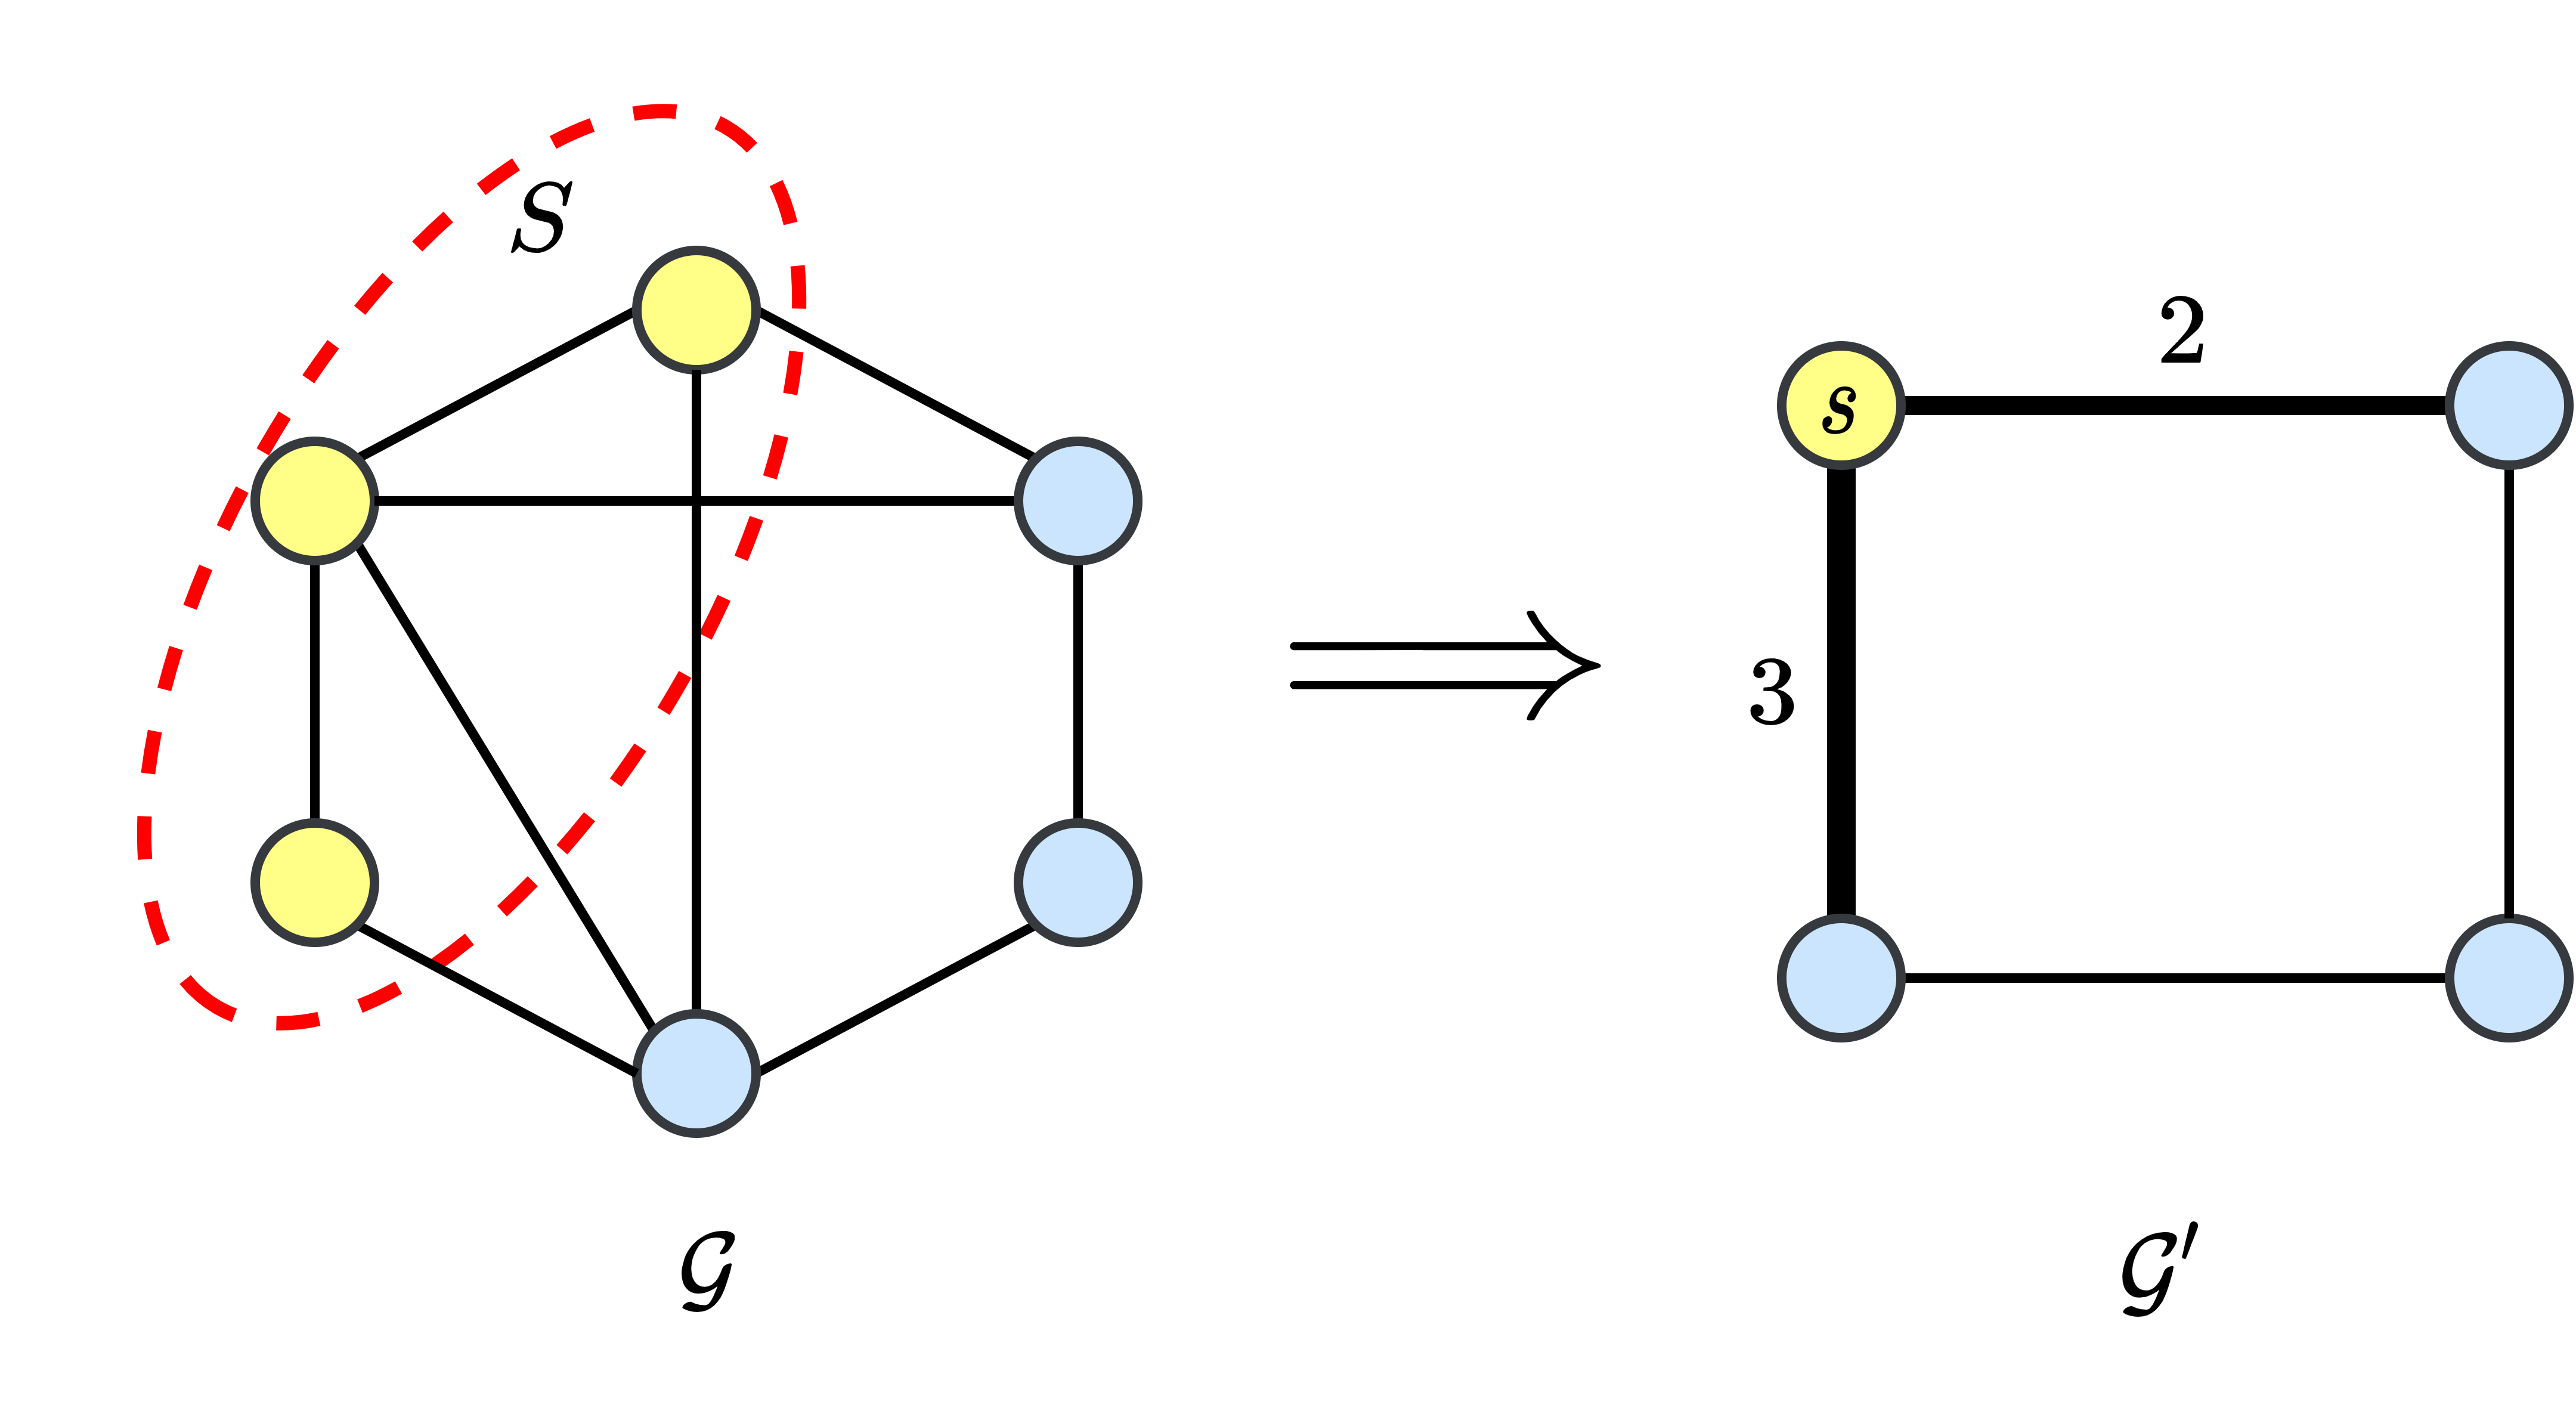
\includegraphics[width=0.9\linewidth]{augmented_graph.png}
        \caption{An example of constructing an augmented graph \(\gr'\) from the original graph \(\gr\), where  vertices in set $S$ are traps. Each edge with a label is an edge with  weight \(1\).}
        \label{fig:augmented-graph}
    \end{figure}

    We proceed to introduce some notation for the augmented graph \(\gr'=\mypar{V',E',w'}\). Let \(d'\) be the sum of the degrees of all vertices in $V'$, let $H'_{ij}$ be the hitting time from vertex $i$ to $j$, and let \(\vecpi'\) be the vector of stationary distribution for random walks on  \(\gr'\). In addition, let $\mathcal{\bar{G}}'=(V',E',w')$ be the electrical network associated with graph \(\gr'=\mypar{V',E',w'}\). Let \(\vcal_i^{sj}\) represent the voltage of vertex \(i\) in the equivalent electrical network $\mathcal{\bar{G}}'$, when a unit current is injected at vertex \(s\) and extracted at vertex \(j\).

    We now establish a link between the GWC \(\manc{S}\) for graph  \(\gr=\mypar{V,E,w}\) and the voltage for the electrical network associated with graph \(\gr'\).

    \begin{theorem}\label{thm:connection-electrical}
        For a vertex group \(S\subseteq V\) in a connected graph \(\gr=(V,E)\), the GWC \(\manc{S}\) can be expressed as
        \begin{equation}\label{eq:connection-electrical}        \manc{S}=d'\sum_{i=1}^{n'}\sum_{j=1}^{n'}\pi'_i\pi'_j\mypar{\vcal_i^{is}+\vcal_i^{sj}-\vcal_i^{ij}}.
        \end{equation}
    \end{theorem}
    \begin{IEEEproof}
        Based on the definition of the augmented graph, the group hitting time and random detour time of \(S\) are equivalent to those of \(s\) in the corresponding augmented graph.
        Then we can rewrite~\eqref{eq:connection-multiple} in \thmref{thm:connection-multiple} as
        \begin{equation}\label{eq:GWC-detour}
            \begin{split}
                \manc{S}&=\sum_{i=1}^n\sum_{j=1}^n\pi_i\pi_jD_{ij}(S)-K\\
                &=\sum_{i=1}^{n'}\sum_{j=1}^{n'}\pi_i\pi_j\mypar{H_{is}+H_{sj}-H_{ij}}.
            \end{split}
        \end{equation}
        According to~\cite{RaZh13},
        \begin{equation}\label{eq:detour-voltage}
            H_{is}+H_{sj}-H_{ij}=d'\mypar{\vcal_i^{is}+\vcal_i^{sj}-\vcal_i^{ij}}.
        \end{equation}
        Combining~\eqref{eq:GWC-detour} and~\eqref{eq:detour-voltage} completes our proof.
    \end{IEEEproof}
\fi

\subsection{Monotonic and Supermodular Properties}

%After proposing physical explanations of GWC, we then attempt to study its properties.
In this subsection, we show that the the set function \(\manc{\cdot}\) has some desirable properties. For this purpose, we first introduce the definitions of monotone and supermodular set functions. For simplicity, we use \(S+u\) to represent \(S\cup\setof{u}\).

\begin{definition}[Monotonicity]
    A set function \(f:2^{V}\to\rea^+\) is monotonic if and only if the inequality \(f(X)\ge f(Y)\) holds for two arbitrary  nonempty sets \(X\) and \(Y\)  satisfying \(X\subseteq Y\subseteq V\).
\end{definition}

\begin{definition}[Supermodularity]
    A set function \(f:2^{V}\to\rea^+\) is  supermodular if and only if the inequality \(f(X)-f(X+u)\ge f(Y)-f(Y+u)\) holds for two arbitrary nonempty sets \(X\) and \(Y\) satisfying \(\forall X\subseteq Y\subseteq V, u\in V\setminus Y\).
\end{definition}

Next we demonstrate that the set function \(\manc{\cdot}\) is  monotonically decreasing and supermodular.

\begin{theorem}\label{thm:mono}
    Let \(S\) be a nonempty set of vertices of a connected weighted undirected graph \(\gr=(V,E,w)\). Then, for any vertex \(u\in V\setminus S\),
    \begin{equation*}
        \manc{S}\ge \manc{S+u}.
    \end{equation*}
\end{theorem}
\begin{IEEEproof}
    By \defref{def:manc}, when a random walker arrives at a vertex in \(S\), it must have arrived at vertices in \(S+u\). Therefore, \(H_{vS}\ge H_{v\mypar{S+u}}\) holds for any vertex \(v\in V\), which concludes our proof.
\end{IEEEproof}

\begin{theorem}\label{thm:supermod}
    Let \(S\) and \(T\) be two  nonempty sets of vertices of a connected weighted undirected graph \(\gr=(V,E,w)\) obeying  \(S\subseteq T\subsetneq V\). Then, for any vertex \(u\in V\setminus T\),
    \begin{equation*}
        \manc{S}-\manc{S+u}\ge \manc{T}-\manc{T+u}.
    \end{equation*}
\end{theorem}
\begin{IEEEproof}
    By definition of absorbing time for  random walks with traps,  \(\manc{S}-\manc{S+u}\) can be represented as
    \begin{equation}\label{eq:supermod-diff}
        \begin{split}
            &\manc{S}-\manc{S+u}\\
            =&\sum_{v\in V}\pi_v\mypar{\mean{T_{vS}}-\mean{T_{v\mypar{S+u}}}}\\
            =&\sum_{v\in V}\pi_v\mypar{\mean{T_{vS}}-\mean{\min\setof{T_{vS},T_{vu}}}}.
        \end{split}
    \end{equation}
    We next represent \(\min\setof{T_{vS},T_{vu}}\)  in terms of  the indicator function.  For a subset \(A\) of the probability space, we denote \(\indfunc{A}\) as the indicator function of the event \(A\). Concretely, \(\indfunc{A}\) is defined as
    \begin{equation*}
        \indfunc{A}=
        \begin{cases}
            1, & \text{event }A\text{ holds true;} \\
            0, & \text{otherwise.}
        \end{cases}.
    \end{equation*}
    Then, \(\min\setof{T_{vS},T_{vu}}\) can
    be recast as
    \begin{equation*}
        \min\setof{T_{vS},T_{vu}}=T_{vS}\indfunc{\setof{T_{vS}\le T_{vu}}}+T_{vu}\indfunc{\setof{T_{vu}<T_{vS}}},
    \end{equation*}
    inserting which into~\eqref{eq:supermod-diff}  and considering  the linearity of the mean, one obtains
    \begin{equation*}
        \manc{S}-\manc{S+u}=\sum_{v\in V}\pi_v\mean{(T_{vS}-T_{vu})\indfunc{\setof{T_{vu}<T_{vS}}}}.
    \end{equation*}
    Similarly, we have
    \[\manc{T}-\manc{T+u}=\sum_{v\in V}\vecpi_v\mean{(T_{vT}-T_{vu})\indfunc{\setof{T_{vu}<T_{vT}}}}.\]
    As mentioned in proof of \thmref{thm:mono}, \(T_{vS}\ge T_{vT}\) holds for any vertex \(v\in V\).
    Thus, when \(T_{vu}<T_{vT}\) holds true, the relation \(T_{vu}<T_{vS}\) also holds.  Then, \(\indfunc{\setof{T_{vu}<T_{vS}}}\ge\indfunc{\setof{T_{vu}<T_{vT}}}\) holds for any vertex \(v\in V\).
    Combining these two inequalities, one obtains
    \[(T_{vS}-T_{vu})\indfunc{\setof{T_{vu}<T_{vS}}}\ge(T_{vT}-T_{vu})\indfunc{\setof{T_{vu}<T_{vT}}}\]
    for any vertex \(v\in V\). This completes the proof.
\end{IEEEproof}


\section{Minimizing  Group Walk Centrality Subject to Cardinality Constraint }

In this section, we define and study the problem of minimizing the GWC \(\manc{S}\) by optimally  selecting a fixed number $k=\abs{S}$ vertices constituting set.

\subsection{Problem Formulation}

As shown above, \(\manc{S}\) is a monotonically deceasing set function, since the addition of any vertex to set $S$ will lead to an decrease of the quantity \(\manc{S}\). Then, we naturally raise the following problem called MinGWC: How to optimally choose a set \(S\) of \(k=\abs{S}\) vertices in graph \(\gr=(V,E)\), so that the quantity \(\manc{S}\) is minimized. Mathematically, the optimization problem subject to a cardinality constraint can be formally stated as follows.

%When considering GWC, we naturally address the issue of selecting a vertex group (\(S\)) with a capacity of \(k\) from a network that minimizes its GWC (\(\manc{S}\)).


\begin{problem}[\underline{Min}imization of \underline{G}roup \underline{W}alk \underline{C}entrality, MinGWC]
Given a connected weighted undirected graph \(\gr=(V,E,w)\) with \(n\) vertices, \(m\) edges and an integer \(k\ll n\), the goal is to find a vertex group \(S^*\subseteq V\) such that the GWC \(\manc{S^*}\) is minimized. In other words,
\begin{equation*}
    S^*=\argmin_{S\subseteq V,\abs{S}=k}\manc{S}.
\end{equation*}
\end{problem}


Since the problem MinGWC is inherently combinatorial, we can naturally resort to a the na\"{\i}ve solution by exhausting all $\tbinom{n}{k}$ cases of vertex selection. For each of the possible cases that $k$ vertices are selected to form set $S$, we calculate the quantity \(\manc{S}\) corresponding to the $k$ vertices in set $S$ and output the optimal solution $S^*$ with the minimum group walk centrality. Evidently, this method fails when $n$ or $k$ is slightly large since it has an exponential time complexity $O(\tbinom{n}{k}n^3)$, assuming that inverting an $n \times n$ matrix needs $O(n^3)$  time. Below we will show that the  MinGWC problem is in fact NP-hard.


\subsection{Hardness of the MinGWC Problem}

In this section, we prove that  the MinGWC problem is NP-hard, by giving a reduction from the vertex cover problem for 3-regular graphs, the vertices of which have identical degree 3. For a 3-regular graph, the vertex cover problem is NP-complete~\cite{FrHeJa98}, the decision version of which is stated below.
\begin{problem}\label{Cover3}
Given a connected 3-regular graph \(G=(V,E)\) and an integer \(k\),  the vertex cover problem is to determine whether exists a subset \(S\subseteq V\) of \(\abs{S}\le k\) vertices, such that every edge in \(E\) is incident with at least one vertex in \(S\), i.e., \(S\) is a vertex cover of \(G=(V,E)\).
\end{problem}

We continue to give a decision version of  the MinGWC problem for a  3-regular graph.
\begin{problem}\label{MinGWC3}
Given a connected 3-regular graph \(G=(V,E)\) with every edge having a unit weight,  an integer \(k\), and a threshold $(n-k)/n$, the MinGWC problem  asks whether exists a subset \(S\subseteq V\) of \(\abs{S}\le k\) vertices, such that \(\manc{S}\ge (n-k)/n\).
\end{problem}




\begin{theorem}\label{thm:np-hard}
    The MinGWC problem is NP-hard.
\end{theorem}
\begin{IEEEproof}
    We give a reduction from the above vertex cover problem in a 3-regular graph  \(G=(V,E)\) to the decision version of the problem of group walk centrality. Specifically, we will prove that for any nonempty set \(S\subseteq V\) of  \(\abs{S}=k\)  vertices, \(\manc{S}\ge (n-k)/n\), where the equality holds if and only if \(S\) is a vertex cover of \(\gr\).


    %For a connected graph \(\gr=(V,E,w)\) that is \(c\)-regular, where the weights of all edges are equal to \(1\), we attempt to prove that \(\manc{S}\ge (n-k)/n\) for any nonempty vertex group \(S\subseteq V\) with capacity \(k\).  The equality holds if and only if \(S\) is a vertex cover of \(\gr\).

    We first prove that if \(S\) is a vertex cover of \(\gr\), then \(\manc{S}=(n-k)/n\). In the case that \(S\) is a vertex cover of \(\gr\), there is no edge between vertices in \(V\setminus S\). Then~\eqref{eq:GWC} is simplified as
    \begin{equation*}
        \manc{S}=\vecpi_{-S}^\top\lap_{-S}^{-1}\vecd_{-S}=\vecpi_{-S}^\top\matd_{-S}^{-1}\vecd_{-S}=\vecpi_{-S}^\top\vecone.
    \end{equation*}
    Since \(\gr\) is a 3-regular graph, \(\vecpi=\begin{pmatrix}1/n&\cdots&1/n\end{pmatrix}^\top\).
    Thus, \(\manc{S}=\vecpi_{-S}^\top\vecone=(n-k)/n\).

    We continue to demonstrate that if \(S\) is not a vertex cover of \(\gr\), then \(\manc{S}>(n-k)/n\).  Note that for the case that \(S\) is not a vertex cover,  for a vertex \(u\in S\) and any vertex \(v\in V\setminus S\), \(H_{uS}=0\) and \(H_{vS}\ge1\) always hold. Moreover, there exists at least one edge \((u',v')\) in edge set \(E\) that is not covered by \(S\). Thus, for a walker starting from vertex \(u'\), it moves to vertex \(v'\) with a probability of at least \(\frac{1}{d_{\max}}>\frac{1}{n}\), then it continue walking until being absorbed by vertices in  \(S\).  For this case the absorbing time $H_{u'S}$ is bounded as
    \begin{align*}
        H_{u'S} & >\mypar{1-\frac{1}{d_{\max}}}\times1+\frac{1}{d_{\max}}\times2  \\
                & >\mypar{1-\frac{1}{n}}\times1+\frac{1}{n}\times2=1+\frac{1}{n}.
    \end{align*}
    Similarly, we obtain \(H_{v'S}>1+\frac{1}{n}\).

    Let \(S'\) denote \(S\cup\setof{u',v'}\). Then we are able to get a lower bound of GWC $\manc{S}$ as
    \begin{align*}
        \manc{S} & =\sum_{v\in V\setminus S'}\pi_vH_{vS}+\pi_{u'}H_{u'S}+\pi_{v'}H_{v'S}            \\
                 & >\vecpi_{-S'}\vecone+\pi_{u'}\mypar{1+\frac{1}{n}}+\pi_{v'}\mypar{1+\frac{1}{n}} \\
                 & =\vecpi_{-S}^\top\vecone+\frac{\pi_{u'}+\pi_{v'}}n
        >\vecpi_{-S}^\top\vecone=(n-k)/n.
    \end{align*}
    This finishes the proof.
    % According to the proposition above, we can create a polynomial reduction from Vertex Cover on \(c\)-regular graphs to a decision version of MinGWC, which proves that MinGWC is NP-hard.
\end{IEEEproof}

\subsection{A Simple Greedy Algorithm}

Since the MinGWC problem is NP-hard, it is nearly impossible to design a polynomial time algorithm to solve it. One often resorts to greedy algorithm. Due to the proved fact that the objective function \(\manc{\cdot}\) of  the MinGWC problem is monotonic and supermodular, a na\"{\i}ve greedy strategy for vertex selection yields an approximated   solution  with a $(1-\frac{k}{k-1}\cdot\frac{1}{e})$ approximation factor~\cite{NeWoFi78}. Initially, we set $S$ to be empty, then $k$ vertices from set $V \setminus S$ are added to $S$ iteratively. During the first iteration, the vertex $u$ with the minimum walk centrality $H_u$ is chosen to be added to $S$. Then, in each iteration step $i>1$, the vertex $u$ in the set $V \setminus S$ of candidate vertices is selected, which has the maximum marginal gain $\Delta(u,S) \triangleq \manc{S}-\manc{S+u}$.  The algorithm terminates when $k$ vertices are chosen to be added to set $S$.

At each iteration of the naive greedy algorithm, one needs computing the maximum marginal gain $\Delta(u,S)$ for every candidate vertex in set $V \setminus S$. As shown in~\eqref{eq:GWC}, a straightforward calculation of  $\Delta(u,S)$ for every vertex \(u\) requires inverting a matrix, which needs $O((n-\abs{S})^3)$ time.  Thus, for the $(O(n-\abs{S}))$ candidate vertices, the computation time at each iteration is $O((n-\abs{S})^4)$. Hence, the total computation complexity of the na\"{\i}ve greedy algorithm is \(O(kn^4)\) since $\abs{S} \ll n$.

\iffalse
    \begin{gather*}
        \Delta(u,S)=\manc{S}-\manc{S+u},\\
        u^*=\argmax_{u\in V\setminus S}\setof{\Delta(u,S)}.
    \end{gather*}
\fi

In order to further decrease the time complexity of the na\"{\i}ve greedy algorithm, we provide an expression for \(\Delta(u,S)\).
\begin{lemma}\label{lem:delta}
    Given a connected weighted undirected graph \(\gr=(V,E,w)\), the nonempty vertex group \(S\), and the Laplacian matrix \(\lap\), for any vertex \(u\in V\setminus S\),  \(\Delta(u,S)\) can be alternatively expressed as
    \begin{equation}\label{eq:delta}
        \Delta(u,S)=   \manc{S}-\manc{S+u}=\frac{\mypar{\vece_u^\top\lap_{-S}^{-1}\vecd_{-S}}^2}{d\mypar{\vece_u^\top\lap_{-S}^{-1}\vece_u}}.
    \end{equation}
\end{lemma}
\begin{IEEEproof}
    For vertex \(u\in V\setminus S\), we denote the \(\myord{u}\) column of submatrix \(\lap_{-S}\) as \(\begin{pmatrix}d_u\\-\veca\end{pmatrix}\). After properly adjusting the vertex labels, matrix \(\lap_{-S}\) can be rewritten  in block form as
    \begin{equation*}
        \lap_{-S}=\begin{pmatrix}d_u & -\veca^\top \\-\veca&\mata\end{pmatrix},
    \end{equation*}
    where \(\mata\) denotes \(\lap_{-(S+u)}\).
    According to the properties of block matrices, we  get
    \begin{equation*}
        \lap_{-S}^{-1}=
        \begin{pmatrix}
            t & t\veca^\top\mata^{-1} \\t\mata^{-1}\veca&\mata^{-1}+t\mata^{-1}\veca\veca^\top\mata^{-1}
        \end{pmatrix},
    \end{equation*}
    where \(t=\pinv{d_u-\veca^\top\inv{\mata}}\).
    Therefore, when \(S\neq\varnothing\), \(\Delta(u,S)\) can be rewritten as
    \begin{equation*}
        \begin{split}
            &\Delta(u,S)=\manc{S}-\manc{S+u}\\
            =&\vecpi_{-S}^\top\lap_{-S}^{-1}\vecd_{-S}-\vecpi_{-(S+u)}^\top\lap_{-(S+u)}^{-1}\vecd_{-(S+u)}\\
            =&\frac1t\mypar{t\vecpi_u+t\vecpi_{-(S+u)}^\top\mata^{-1}\veca}\mypar{td_u+t\veca^\top\mata^{-1}\vecd_{-(S+u)}}\\       =&\frac{\mypar{\vecpi_{-S}^\top\lap_{-S}^{-1}\vece_u}\mypar{\vece_u^\top\lap_{-S}^{-1}\vecd_{-S}}}{\vece_u^\top\lap_{-S}^{-1}\vece_u}=\frac{\mypar{\vece_u^\top\lap_{-S}^{-1}\vecd_{-S}}^2}{d\mypar{\vece_u^\top\lap_{-S}^{-1}\vece_u}},
        \end{split}
    \end{equation*}
    finishing the proof.
\end{IEEEproof}


\lemref{lem:delta} demonstrate that for any empty set $S$ if \(\lap_{-S}\)  is already computed, by using~\eqref{eq:delta}  we can calculate \(\Delta(u,S)\) for any vertex \(u\in V\setminus S\) in $O((n-\abs{S})^2)$ time.
This avoids directly inverting the matrix \(\lap_{-(S+u)}\), which needs time $O((n-\abs{S}+1)^3)$. When \(S=\varnothing\),~\eqref{eq:delta} becomes invalid.  For this case, we use the result \(H_u=d\mypar{\vece_u-\vecpi}^\top\lap^{\dagger}\mypar{\vece_u-\vecpi}\) in~\lemref{HjK} to compute the walk centrality $H_u$ for every vertex $u \in V$, and add the vertex $u$ with the smallest $H_u$ to $S$.  Based on~\lemref{HjK} and~\lemref{lem:delta}, we propose a simple greedy algorithm \textsc{DeterMinGWC}$(\gr,k)$ to solve the MinGWC problem, which is  outlined in~\algoref{algo:exact-gwcm}. The algorithm first computes $H_u$ for every vertex $u \in V$ in time $O(n^3)$. Then, it works in $k-1$ rounds. In each round, it evaluates  \(\Delta(u,S)\) for all the $ (n-\abs{S})$ vertices in set $V \setminus S$ (Line 6)  in $O((n-\abs{S})^3)$ time. Therefore, the whole running time of~\algoref{algo:exact-gwcm} is \(O(kn^3)\),  much lower than the time complexity   \(O(kn^4)\) of the  na\"{\i}ve greedy  algorithm.


\begin{algorithm}
    \caption{\textsc{DeterMinGWC}\((\gr,k)\)}
    \label{algo:exact-gwcm}
    \Input{
        A connected weighted undirected graph \(\gr=(V,E,w)\);
        an integer \(k \ll \abs{V}\)
    }
    \Output{\(S_k\): A subset of \(V\) with \(\abs{S_k}=k\)}
    Compute \(\lap\) and \(\vecd\)\;
    \(d\gets\vecd\vecone\),\(\vecpi\gets \inv{d}\vecd\)\;
    \(S_1\gets\setof{\argmin_{u\in V}\setof{d(\vece_u-\vecpi)^\top\lap^\dagger(\vece_u-\vecpi)}}\)\;
    \For{\(i=2,3,\dots,k\)}{
        \ForEach{\(u\in V\setminus S\)}{
            \(\Delta(u,S)\gets\frac{(\vece_u^\top\lap_{-S}^{-1}\vecd_{-S})^2}{d(\vece_u^\top\lap_{-S}^{-1}\vece_u)}\)\;
        }
        \(u^*\gets\argmax_{u\in V\setminus S}\setof{\Delta(u,S)}\)\;
        \(S_i\gets S_{i-1}\cup\setof{u^*}\)
    }
    \Return{\(S_k\)}
\end{algorithm}

In addition to good efficiency, \algoref{algo:exact-gwcm} is very effective since it has a $(1-\frac{k}{k-1}\cdot\frac{1}{e})$ approximation factor, as shown in the following theorem.
\begin{theorem}
    The algorithm $S_k$= \textsc {DeterMinGWC}$ (\gr,k)$ takes a connected weighted undirected graph \(\gr=(V,E,w)\) and a positive integer \(1 \geq k \ll n\), and returns a  group \(S_k\) of \(k\) vertices.
    The return vertex group \(S\) satisfies
    \[\manc{\setof{u^*}}-\manc{S_k}\ge\mypar{1-\frac{k}{k-1}\cdot\frac{1}{e}}\mypar{\manc{\setof{u^*}}-\manc{S^*}},\]
    where
    \[u^*\defeq\argmin_{u\in V}\manc{\setof{u}}\] and \[S^*\defeq\argmin_{\abs{S}=k}\manc{S}.\]
\end{theorem}
\begin{IEEEproof}
    According to the supermodularity of \(\manc{\cdot}\),
    \[\manc{S_i}-\manc{S_{i+1}}\ge\frac{1}{k}\mypar{\manc{S_i}-\manc{S^*}}\]
    holds for any positive integer \(i\), which indicates
    \[\manc{S_{i+1}}-\manc{S^*}\le\mypar{1-\frac{1}{k}}\mypar{\manc{S_i}-\manc{S^*}}.\]
    Then, we  further obtain
    \begin{align*}
        \manc{S_k}-\manc{S^*}\le & \mypar{1-\frac{1}{k}}^{k-1}\mypar{\manc{S_1}-\manc{S^*}}    \\
        \le                      & \frac{k}{k-1}\cdot\frac{1}{e}\mypar{\manc{S_1}-\manc{S^*}},
    \end{align*}
    which, together with the fact that \(S_1=\setof{u^*}\), completes the proof.
\end{IEEEproof}

\section{Fast Greedy Algorithm for the MinGWC Problem}\label{sec:approx-algo2}

Although \algoref{algo:exact-gwcm} is much faster than the  na\"{\i}ve greedy  algorithm, it  still cannot handle  large networks since its time complexity is  \(O(kn^3)\). As shown above, the key steps for \algoref{algo:exact-gwcm} are  to compute the walk centrality $H_u$ for every vertex $u \in V$ and the marginal gain  \(\Delta(u,S)\) for every vertex $u \in (V \setminus S)$. In this section, we provide efficient approximations for  $H_u$ and \(\Delta(u,S)\). For $H_u$, it can be efficiently evaluated by using \algoref{ALG01}. For \(\Delta(u,S)\), we can alternatively approximate the two quantities  $\vece_u^\top \lap_{-S}^{-1} \vecd_{-S}$ and $\vece_u^\top \lap_{-S}^{-1}\vece_u$ in the numerator and denominator of~\eqref{eq:delta}, respectively.

In the rest of this section, we first approximate $\vece_u^\top \lap_{-S}^{-1} \vecd_{-S}$ and $\vece_u^\top \lap_{-S}^{-1}\vece_u$. Then, we present an  error-guaranteed approximation to  \(\Delta(u,S)\), based on which we further propose  a fast approximation algorithm to the MinGWC problem  with $(1-\frac{k}{k-1} \frac{1}{e}-\epsilon)$ approximation ratio and time complexity $\tilde{O}(km\epsilon^{-2})$ for any error parameter $0< \epsilon < 1$.


\subsection{Approximation of the Quantity $\mathbf{e}_i^\top \mathbf{L}_{-S}^{-1}\mathbf{e}_S$}

We first  approximate the quantity \(\vece_i^\top\lap_{-S}^{-1}\vecd_{-S}\) for any node $i\in V\setminus S$. To this end, we introduce the following two lemmas.
\begin{lemma}\label{lem:norm-ineq}
    Let \(\gr=(V,E,w)\) be a connected weighted undirected graph with Laplacian matrix  \(\lap\). Then, for an arbitrary subset \(S\subseteq V\) of vertices and an arbitrary vector \(\vecv\in\rea^{n-\abs{S}}\), the relation \(v_i^2\le nw_{\min}^{-1}\Abs{\vecv}^2_{\lap_{-S}}\) holds.
\end{lemma}
\begin{IEEEproof}
    As shown in~\secref{sub:lap}, Laplacian matrix $\lap$ can be written as \(\lap=\matb^\top\matw\matb\).   Similarly, as an SDDM matrix, \(\lap_{-S}\) can be decomposed as \(\lap_{-S}=\lap'+\matz=\matb'^\top\matw'\matb'+\matz\), where \(\lap'\) denotes the Laplacian matrix of a  graph, and \(\matz\) is a diagonal matrix with every diagonal entry  larger than 0. In order to prove the lemma, we distinguish two cases:  \(\matz_{[i,i]}\neq0\) and  \(\matz_{[i,i]}=0\).

    For the first case \(\matz_{[i,i]}\neq0\),  we have \(\matz_{[i,i]}\ge w_{\min}\). Then, it is apparent that \(v_i^2\le nw_{\min}^{-1}\Abs{\vecv}^2_{\lap_{-S}}\). For the second case  \(\matz_{[i,i]}=0\), there must exist a vertex \(j\)  satisfying \(\matz_{[j,j]}\ge w_{\min}\) in a component of the resultant graph containing vertex \(i\), which is obtained from \(\gr=(V,E,w)\) after removing vertices in \(S\).    Let \(\pscr_{ij}\) denotes a simple path connecting vertex \(i\) and vertex \(j\). Then, we have
    \begin{align*}
        \Abs{\vecv}^2_{\lap_{-S}}
         & \ge w_{\min}\sum_{\edge{a}{b}\in\pscr_{ij}}(v_a-v_b)^2+w_{\min}v_j^2     \\
         & \ge w_{\min}n^{-1}\mypar{\sum_{\edge{a}{b}\in\pscr_{ij}}(v_a-v_b)+v_j}^2 \\
         & \ge w_{\min}n^{-1}v_i^2,
    \end{align*}
    which completes our proof.
\end{IEEEproof}


\begin{lemma}\label{lem:trace-lap}
    Let \(\gr=(V,E,w)\) be a connected weighted undirected graph with \(n\) vertices and the minimum edge weight $ w_{\min}$, and let \(\lap\) be the Laplacian matrix of \(\gr\). Then, for any nonempty set \(S\subseteq V\),
    \begin{equation*}
        \trace{\lap_{-S}^{-1}}\le n^2w_{\min}^{-1}.
    \end{equation*}
\end{lemma}
\begin{IEEEproof}
    According to the result in~\cite{ClPo11}, the diagonal entry \(\mypar{\lap_{-S}}_{[u,u]}\) of \(\lap_{-S}\) is exactly the resistance distance \(R_{uS}\) between vertex \(u\) and vertex group \(S\).  Since \(\gr\) is connected, the length of an arbitrary simple path connecting vertex \(u\) any vertex in \(S\) is no more than \(n\).
    Making use of~\eqref{eq:phy-resist}, we have
    \begin{align*}
        \trace{\lap_{-S}^{-1}} & =\sum_{i=1}^n\vece_i^\top\lap_{-S}^{-1}\vece_i=\sum_{i=1}^nR_{iS}              \\
                               & \le\sum_{i=1}^n\sum_{\edge{a}{b}\in\pscr_{iS}}w_{ab}^{-1}\le n^2w_{\min}^{-1},
    \end{align*}
    which finishes the proof.
\end{IEEEproof}

With the above two lemmas, we can approximate \(\vece_u^\top\lap_{-S}^{-1}\vecd_{-S}\). For simplicity of the following proofs, define $\vecx_i $ as \(\vecx_i=\vece_i^\top\lap_{-S}^{-1}\vecd_{-S}\) for any vertex \(i\in V\setminus S\). By definition, $\vecx_i $ represents the trapping time of a random walker starting at vertex \(i\) and being absorbed by  vertices in $S$. Then, it follows that \(\vecx_i\ge1\). Since \(\lap_{-S}\) is an SDDM matrix, we can estimate $\vecx_i $ by applying~\lemref{lemma:ST}, which avoids computing the inverse of matrix \(\lap_{-S}^{-1}\).

\begin{lemma}\label{lem:approx-numer}
    Let \(\gr=(V,E,w)\) be a connected weighted undirected graph with the Laplacian matrix \(\lap\). Let  \(S\) be a nonempty subset of vertex set $V$, let $\epsilon$ an error parameter in  $(0,1)$, and let \(\vecx'=\mathtt{Solver}(\lap_{-S},\vecd_{-S},\delta_1)\), where \(\delta_1=\frac{w_{\min}\epsilon}{7n^3w_{\max}}\). Then, for any vertex \(i\in V\setminus S\),
    \begin{equation}\label{eq:approx-numer}
        \vecx_i=\vece_i^\top\lap_{-S}^{-1}\vecd_{-S}\approx_{\epsilon/7}\vecx'_i.
    \end{equation}
\end{lemma}
\begin{IEEEproof}
    Combining \lemref{lemma:ST} and \lemref{lem:norm-ineq}, \((\vecx'_i-\vecx_i)^2\) is bounded  as
    \begin{align*}
        (\vecx'_i-\vecx_i)^2
         & \le nw_{\min}^{-1}\Abs{\vecx'-\vecx}^2_{\lap_{-S}}
        \le nw_{\min}^{-1}\delta_1^2\Abs{\vecx}^2_{\lap_{-S}}        \\
         & \le n^4w_{\min}^{-1}w_{\max}^2\delta_1^2\trace{\lap_{-S}}
        \le n^6w_{\min}^{-2}w_{\max}^2\delta_1^2,
    \end{align*}
    where the last inequality is due to \lemref{lem:trace-lap}.
    Considering \(\vecx_i\ge1\), we obtain
    \begin{equation*}
        \frac{\abs{\vecx'_i-\vecx_i}}{\vecx_i}\le n^3w_{\max}w_{\min}^{-1}\delta_1=\epsilon/7,
    \end{equation*}
    which leads to the desirable  result.
\end{IEEEproof}


%\subsection{Approximation of the denominator  of \(\Delta(u,S)\)}

\subsection{Approximation of the Quantity $\mathbf{e}_i^\top \mathbf{L}_{-S}^{-1}\mathbf{e}_i$}

We next estimate the quantity $\mathbf{e}_i^\top \mathbf{L}_{-S}^{-1}\mathbf{e}_i$ in the denominator  of~\eqref{eq:delta}. For this purpose,
we represent $\mathbf{e}_i^\top \mathbf{L}_{-S}^{-1}\mathbf{e}_i$ in terms of an Euclidean norm as
\begin{equation}\label{eq:denom-solver}
    \begin{split}
        & \vece_i^\top\lap_{-S}^{-1}\vece_i
        =\vece_i^\top\lap_{-S}^{-1}(\matb'^\top\matw'\matb'+\matz)\lap_{-S}^{-1}\vece_i\\
        =&\vece_i^\top\lap_{-S}^{-1}\matb'^\top\matw'\matb'\lap_{-S}^{-1}\vece_i+\vece_i^\top\lap_{-S}^{-1}\matz\lap_{-S}^{-1}\vece_i\\
        =&\Abs{\matw'^{1/2}\matb'\lap_{-S}^{-1}\vece_i}^2+\Abs{\matz^{1/2}\lap_{-S}^{-1}\vece_i}^2.
    \end{split}
\end{equation}
Thus, the evaluation of $\mathbf{e}_i^\top \mathbf{L}_{-S}^{-1}\mathbf{e}_i$ is reduced to computing  the $\ell_2$-norm of two vectors in $\rea^m$ and $\rea^n$, respectively. However, exactly calculating $\mathbf{e}_i^\top \mathbf{L}_{-S}^{-1}\mathbf{e}_i$ by evaluating $\ell_2$-norms still has a high computational cost, since we still need to invert the matrix  $\mathbf{L}_{-S}$. Although by utilizing \lemref{lemma:ST}, one can approximate $\ell_2$-norms. Unfortunately,  since the dimensions of matrices \(\matw'\) and \(\matz\) are, respectively,  $O(m)$ and  $O(n)$, resulting in an unacceptable number of calls to the \(\mathtt{Solver}\) function. In the following text, by using~\lemref{lemma:JL} we will propose an approximating algorithm to estimate the two $\ell_2$-norms, which significantly lessens the computational cost.

In order to exploit \lemref{lemma:JL}, we introduce two projection matrices \(\matq\in\rea^{q\times m}\) and \(\matr\in\rea^{r\times n}\), where \(q=r=\ceil{24\epsilon^{-2}\log n}\). Each of the entry for \(\matq\in\rea^{q\times m}\) and \(\matr\in\rea^{r\times n}\) is  $1/\sqrt{q}$ or $1/\sqrt{q}$ with identical probability $1/2$. Then, we have
\begin{equation}\label{eq:denom-jl}
    \begin{split}
        &\mathbf{e}_i^\top \mathbf{L}_{-S}^{-1}\mathbf{e}_i =\Abs{\matw'^{1/2}\matb'\lap_{-S}^{-1}\vece_i}^2+\Abs{\matz^{1/2}\lap_{-S}^{-1}\vece_i}^2\\
        \approx_\epsilon&\Abs{\matq\matw'^{1/2}\matb'\lap_{-S}^{-1}\vece_i}^2+\Abs{\matr\matz^{1/2}\lap_{-S}^{-1}\vece_i}^2.
    \end{split}
\end{equation}
For the sake of simplicity, we denote \(\matw'^{1/2}\matb'\lap_{-S}^{-1}\) and \(\matq\matw'^{1/2}\matb'\lap_{-S}^{-1}\) as \(\matx\) and \(\tilde{\matx}\), respectively. Moreover, we  denote \(\matz^{1/2}\lap_{-S}^{-1}\) and \(\matr\matz^{1/2}\lap_{-S}^{-1}\) as \(\maty\) and \(\tilde{\maty}\), respectively.
Then~\eqref{eq:denom-jl} can be rephrased as
\begin{equation}\label{eq:denom-solver-simp}
    \begin{split}
        \vece_i^\top\lap_{-S}^{-1}\vece_i &=\Abs{\matx\vece_i}^2+\Abs{\maty\vece_i}^2\\
        &\approx_\epsilon\Abs{\tilde{\matx}\vece_i}^2+\Abs{\tilde{\maty}\vece_i}^2.
    \end{split}
\end{equation}
Making this expression,  we can efficiently approximate the quantity $\vece_i^\top\lap_{-S}^{-1}\vece_i$.

\begin{lemma}\label{lem:approx-denom}
    Let \(\gr=(V,E,w)\) be a connected weighted undirected graph with Laplacian matrix \(\lap\). Let  \(S\) be a nonempty subset of vertex set $V$, and let  $\epsilon$ be an error parameter in $(0,1)$. Let  \(\overline{\matx}\) and \(\overline{\maty}\)   denote \(\matq\matw^{1/2}\matb\) and \(\matr\matz^{1/2}\) respectively.   Let \(\matx'\in\rea^{q\times n}\) and \(\maty'\in\rea^{r\times n}\) be matrices such that \(\matx'_{[i,:]}=\mathtt{Solver}(\lap_{-S},\overline{\matx}_{[i,:]},\delta_2)\), \(\maty'_{[i,:]}=\mathtt{Solver}(\lap_{-S},\overline{\maty}_{[i,:]},\delta_2)\), where \(q=r=\ceil{24(\epsilon/7)^{-1}}\log n\), \(\delta_2=\frac{w_{\min}\epsilon}{31n^2}\sqrt{\frac{1-\epsilon/7}{2w_{\max}(1+\epsilon/7)}}\). Then, for any vertex \(i\in V\setminus S\),
    \begin{equation}\label{eq:approx-denom}
        \vece_i^\top\lap_{-S}^{-1}\vece_i = \Abs{\matx\vece_i}^2+\Abs{\maty\vece_i}^2 \approx_{\epsilon/3}\Abs{\matx'\vece_i}^2+\Abs{\maty'\vece_i}^2.
    \end{equation}
\end{lemma}
\begin{IEEEproof}
    According to triangle inequality, we have
    \begin{align*}
            & \abs{\Abs{\tilde{\matx}\vece_i}-\Abs{\matx'\vece_i}}\le\Abs{(\tilde{\matx}-\matx)\vece_i}                                                   \\
        \le & \Abs{\tilde{\matx}-\matx'}_{F}= \sqrt{\sum_{j=1}^q\Abs{\tilde{\matx}_{[j,:]}-\matx'_{[j,:]}}^2}                                             \\
        \le & \sqrt{\sum_{j=1}^qnw_{\min}^{-1}\Abs{\tilde{\matx}_{[j,:]}-\matx'_{[j,:]}}_{\lap_{-S}}^2}                                                   \\
        \le & \sqrt{\sum_{j=1}^qnw_{\min}^{-1}\delta_2^2\Abs{\tilde{\matx}_{[j,:]}}_{\lap_{-S}}^2}\le n\delta_2\sqrt{w_{\min}^{-1}}\Abs{\tilde{\matx}}_F,
    \end{align*}
    where the third inequality and the fourth inequality are due to \lemref{lem:norm-ineq} and \lemref{lemma:ST}, respectively.

    Considering \(q=r=\ceil{24(\epsilon/7)^{-1}}\log n\) and~\lemref{lemma:JL}, we further obtain
    \begin{align*}
            & n\delta_2\sqrt{w_{\min}^{-1}}\Abs{\tilde{\matx}}_F\le n\delta_2\sqrt{w_{\min}^{-1}(1+\epsilon/7)\sum_{i\in V\setminus S}\Abs{\matx\vece_i}^2} \\
        \le & n\delta_2\sqrt{w_{\min}^{-1}(1+\epsilon/7)\trace{\lap_{-S}^{-1}}}\le n^2\delta_2w_{\min}^{-1}\sqrt{1+\epsilon/7},
    \end{align*}
    where the last inequality is due to \lemref{lem:trace-lap}.
    Similarly, for \(\abs{\Abs{\tilde{\maty}\vece_i}-\Abs{\maty'\vece_i}}\), we have
    \begin{equation}\label{eq:approx-maty-raw}
        \abs{\Abs{\tilde{\maty}\vece_i}-\Abs{\maty'\vece_i}}\le n^2\delta_2w_{\min}^{-1}\sqrt{1+\epsilon/7}.
    \end{equation}
    On the other hand, according to \lemref{lemma:JL}, we have
    \[\Abs{\tilde{\matx}\vece_i}^2+\Abs{\tilde{\maty}\vece_i}^2\ge(1-\epsilon/7)\vece_i^\top\lap_{-S}^{-1}\vece_i\ge(1-\epsilon/7)n^{-2}w_{\max}^{-1}\]
    where the last inequality is due to the scaling of \(\vece_i^\top\lap_{-S}^{-1}\vecd_{-S}\ge1\).

    According to the Pigeonhole Principle, at least one element of \(\setof{\Abs{\tilde{\matx}\vece_i},\Abs{\tilde{\maty}\vece_i}}\) is no less than \(\frac{1}{n}\sqrt{\frac{1-\epsilon/7}{2w_{\max}}}\).
    Without loss of generality, we suppose \(\Abs{\tilde{\matx}\vece_i}\ge\frac{1}{n}\sqrt{\frac{1-\epsilon/7}{2w_{\max}}}\). Then, we have
    \[\frac{\abs{\Abs{\tilde{\matx}\vece_i}-\Abs{\matx'\vece_i}}}{\Abs{\tilde{\matx}\vece_i}}\le n\delta_2w_{\min}^{-1}\sqrt{\frac{2w_{\max}(1+\epsilon/7)}{1-\epsilon/7}}=\frac{\epsilon}{31}.\]
    In addition, we obtain
    \begin{align*}
            & \frac{\abs{\Abs{\tilde{\matx}\vece_i}^2-\Abs{\matx'\vece_i}^2}}{\Abs{\tilde{\matx}\vece_i}^2}                                                   \\
        =   & \frac{\abs{\Abs{\tilde{\matx}\vece_i}-\Abs{\matx'\vece_i}}\mypar{\Abs{\tilde{\matx}\vece_i}+\Abs{\matx'\vece_i}}}{\Abs{\tilde{\matx}\vece_i}^2} \\
        \le & \frac{\epsilon}{31}\mypar{2+\frac{\epsilon}{31}}\le\frac{\epsilon}{15},
    \end{align*}
    which means
    \begin{equation}\label{eq:approx-matx}
        \frac{\abs{\Abs{\tilde{\matx}\vece_i}^2-\Abs{\matx'\vece_i}^2}}{\Abs{\tilde{\matx}\vece_i}^2+\Abs{\tilde{\maty}\vece_i}^2}\le\frac{\abs{\Abs{\tilde{\matx}\vece_i}^2-\Abs{\matx'\vece_i}^2}}{\Abs{\tilde{\matx}\vece_i}^2}\le\frac{\epsilon}{15}.
    \end{equation}
    Using~\eqref{eq:approx-maty-raw}, it is not difficult to  obtain
    \[\frac{\abs{\Abs{\tilde{\maty}\vece_i}-\Abs{\maty'\vece_i}}}{\Abs{\tilde{\matx}\vece_i}}\le n\delta_2w_{\min}^{-1}\sqrt{\frac{2w_{\max}(1+\epsilon/7)}{1-\epsilon/7}}=\frac{\epsilon}{31},\]
    which indicates
    \begin{equation}\label{eq:approx-maty}
        \begin{split}
            &\frac{\abs{\Abs{\tilde{\maty}\vece_i}^2-\Abs{\maty'\vece_i}^2}}{\Abs{\tilde{\matx}\vece_i}^2+\Abs{\tilde{\maty}\vece_i}^2}\\
            \le&\frac{\abs{\Abs{\tilde{\maty}\vece_i}-\Abs{\maty'\vece_i}}\mypar{\Abs{\tilde{\maty}\vece_i}+\Abs{\maty'\vece_i}}}{\Abs{\tilde{\matx}\vece_i}^2}\\
            \le&\frac{\epsilon}{31}\mypar{2+\frac{\epsilon}{31}}\le\frac{\epsilon}{15}.
        \end{split}
    \end{equation}
    Combining~\eqref{eq:approx-matx} and~\eqref{eq:approx-maty}, we are finally able to get
    \begin{align*}
            & \frac{\abs{\mypar{\Abs{\matx'\vece_i}^2+\Abs{\maty'\vece_i}^2}-\mypar{\Abs{\tilde{\matx}\vece_i}^2+\Abs{\tilde{\maty}\vece_i}^2}}}{\Abs{\matx'\vece_i}^2+\Abs{\maty'\vece_i}^2}             \\
        \le & \frac{\abs{\Abs{\tilde{\matx}\vece_i}^2-\Abs{\matx'\vece_i}^2}+\abs{\Abs{\tilde{\maty}\vece_i}^2-\Abs{\maty'\vece_i}^2}}{\Abs{\matx'\vece_i}^2+\Abs{\maty'\vece_i}^2}\le\frac{\epsilon}{7},
    \end{align*}
    which, together with~\lemref{lemma:JL}, completes the proof.
\end{IEEEproof}



\subsection{Efficient Evaluation of Marginal Gain \(\Delta(u,S)\)}

Combining Lemmas~\ref{lem:approx-numer} and~\ref{lem:approx-denom}, we propose an efficient algorithm called \text{ApproxDelta} approximating \(\Delta(u,S)\) for  \(S\neq\varnothing\). The outline of  \text{ApproxDelta} is presented in Algorithm~\ref{algo:approxdelta}. The \text{ApproxDelta} algorithm calls the \(\mathtt{Solver}\) in \lemref{lem:approx-denom} for \(q=\ceil{24(\epsilon/7)^{-2}\log n}\) times, resulting in a complexity of \(\tilde{O}\mypar{m\epsilon^{-2}}\). The approximation guarantee for Algorithm~\ref{algo:approxdelta} is provided in
Lemma~\ref{lem:approx-marginest}.


\begin{algorithm}
    \caption{\textsc{ApproxDelta}\((\gr,S,\epsilon)\)}
    \label{algo:approxdelta}
    \Input{
        \(\gr=(V,E,w)\): a connected weighted undirected graph;
        \(S\subseteq V\): the absorbing vertex set;
        \(\epsilon\in(0,1)\): an approximation parameter
    }
    \Output{
        \(\Delta(u,S)\): the margin for vertex \(u\in V\setminus S\)
    }
    \(\lap=\) Laplacian of \(\gr\), \(d_u=\) the degree of \(u\) for all \(u\in V\), \(d=\sum_{u \in V} d_u\)\;
    \(n=\abs{V},m=\abs{E}\)\;
    \(w_{\min}=\min\setof{w_e|e\in E},w_{\max}=\max\setof{w_e|e\in E}\)\;
    \(\delta_1= \frac{w_{\min}\epsilon}{7n^2w_{\max}}\),\(\delta_2= \frac{w_{\min}\epsilon}{31n^2}\sqrt{\frac{1-\epsilon/7}{2w_{\max}(1+\epsilon/7)}}\)\;
    \(\vecx'=\mathtt{Solver}(\lap_{-S},\vecd_{-S},\delta_1)\)\;
    Construct matrix \(\matq_{q\times m}\) and \(\matr_{q\times n}\), where \(q=\ceil{24(\epsilon/7)^{-2}\log n}\) and each entry is \(\pm 1/\sqrt{q}\) with identical probability\;
    Decompose \(\lap_{-S}\) into \(\matb'\in\rea^{m\times n}\), \(\matw'\in\rea^{m\times m}\) and \(\matz\in\rea^{n\times n}\), satisfying \(\lap_{-S}=\matb'^\top\matw'\matb'+\matz\)\;
    \(\overline{\matx}=\matq\matw^{1/2}\matb\),\(\overline{\maty}=\matr\matz^{1/2}\)\;
    \For{\(i=1\) to \(q\)}{
    \(\matx'_{[i,:]}=\mathtt{Solver}(\lap_{-S},\overline{\matx}_{[i,:]},\delta_2)\)\;
    \(\maty'_{[i,:]}=\mathtt{Solver}(\lap_{-S},\overline{\maty}_{[i,:]},\delta_2)\)\;
    }
    \ForEach{\(u\in V\setminus S\)}{
        \(\Delta'(u,S)=\frac{\vecx'^2}{d\mypar{\Abs{\matx'\vece_i}^2+\Abs{\maty'\vece_i}^2}}\)\;
    }
    \Return{\(\setof{\Delta'(u,S)|u\in V\setminus S}\)}

\end{algorithm}

\begin{lemma}\label{lem:approx-marginest}
    For any real number \(\epsilon\in(0,1)\), the returned value \(\Delta'(u,S)\) of Algorithm~\ref{algo:approxdelta} satisfies
    \begin{equation*}
        \Delta(u,S)\approx_\epsilon \Delta'(u,S)
    \end{equation*}
    with high probability.
\end{lemma}
% \begin{IEEEproof}

% \end{IEEEproof}





\subsection{Nearly Linear Algorithm for the MinGWC Problem}

By combining \algoref{ALG01} and \algoref{algo:approxdelta}, we develop a faster greedy approximation algorithm called \(\textsc{ApproxMinGWC}\), outlined in Algorithm~\ref{algo:approx}. The algorithm has time  complexity \(\tilde{O}\mypar{km\epsilon^{-2}}\), which  is nearly linear in $m$,  since it calls \textsc{ApproxHK} once and \textsc{ApproxDelta} \(k-1\) times. Algorithm~\ref{algo:approx} has a $(1-\frac{k}{k-1}\cdot\frac{1}{e}-\epsilon)$ approximation factor, as shown in Theorem~\ref{Mainthm}.

\begin{algorithm}
    \caption{\textsc{ApproxMinGWC}\((\gr,k,\epsilon)\)}
    \label{algo:approx}
    \Input{
        \(\gr=(V,E,w)\): a connected weighted undirected graph;
        \(k\ll\abs{V}\): the capacity of vertex set;
        \(\epsilon\in(0,1)\): an approximation parameter
    }
    \Output{\(S_k\): A subset of \(V\) with \(\abs{S_k}=k\)}
    \(\setof{\tilde{H}_u|u\in V }=\textsc{ApproxHK}(\gr,\epsilon)\)\;
    \(S_1=\setof{\argmin_{u\in V}\setof{\tilde{H}_u}}\)\;
    \For{\(i=2\) to \(k\)}{
        \(\setof{\Delta'(u,S)|u\in V\setminus S}=\textsc{ApproxDelta}(\gr,S,\epsilon)\)\;
        \(u^*=\argmax_{u\in V\setminus S}\setof{\Delta'(u,S)}\)\;
        \(S_i= S_{i-1}\cup\setof{u^*}\)\;
    }
    \Return{\(S_k\)}
\end{algorithm}

\begin{theorem}\label{Mainthm}
    The algorithm \(\textsc{ApproxMinGWC}(\gr,k,\epsilon)\) takes a connected weighted undirected graph \(\gr=(V,E,w)\) with Laplacian matrix \(\lap\) , a positive integer \(1<k \ll n\), and an error parameter \(\epsilon\in(0,1)\), and returns a set  \(S_k\) of \(k\) vertices. With high probability, the returned vertex set \(S\) satisfies
    \begin{align*}
        \mypar{1+\epsilon} & \manc{\setof{u^*}}-\manc{S_k}\ge                                                                         \\
                           & \mypar{1-\frac{k}{k-1}\cdot\frac{1}{e}-\epsilon}\mypar{\mypar{1+\epsilon}\manc{\setof{u^*}}-\manc{S^*}},
    \end{align*}
    where
    \[u^*\defeq\argmin_{u\in V}\manc{\setof{u}}, S^*\defeq\argmin_{\abs{S}=k}\manc{S}.\]
\end{theorem}
\begin{IEEEproof}
    Considering~\lemref{lem:approx-marginest} and the supermodular property of the objective function $H(\cdot)$, we are able to obtain  that for any positive integer \(i\),
    \begin{equation*}
        \manc{S_i}-\manc{S_{i+1}}\ge\frac{1-\epsilon}{k}\mypar{\manc{S_i}-\manc{S^*}},
    \end{equation*}
    which indicates
    \begin{equation*}
        \manc{S_{i+1}}-\manc{S^*}\le\mypar{1-\frac{1-\epsilon}{k}}\mypar{\manc{S_i}-\manc{S^*}}.
    \end{equation*}
    % By Theorem~\ref{TheoAlg1}, 
    Repeating the above process, we  further obtain
    \begin{align*}
        \manc{S_k}-\manc{S^*} \le & \mypar{1-\frac{1-\epsilon}{k}}^{k-1}\mypar{\manc{S_1}-\manc{S^*}}            \\
        \le                       & \mypar{\frac{k}{k-1}\cdot\frac{1}{e}+\epsilon}\mypar{\manc{S_1}-\manc{S^*}},
    \end{align*}
    which, together with  the fact that \(\manc{S_1}\le\mypar{1+\epsilon}\manc{\setof{u^*}}\),
    completes the proof.
\end{IEEEproof}


\section{Numerical Experiments}

In this section, we present experimental results for various real and model networks to demonstrate the  efficiency and accuracy of our  approximation algorithms:  \textsc{ApproxHK} for computing the walk centrality \(H_u\) of  every vertex $u$ and the Kemeny constant \(K\), \textsc{DeterMinGWC} and \textsc{ApproxMinGWC} for solving the problem of Minimizing GWC.


\subsection{Experimental Settings}

\textbf{Datasets.} The data of realistic networks are taken from the Koblenz Network Collection~\cite{Ku13} and SNAP~\cite{LeKr14}. For those networks that are disconnected originally, we perform our experiments on their largest connected components (LCC). Related information about the number of vertices and edges for the studied real networks and their LCC is shown  in \tabref{tab:runtime_comparison},  where networks are listed in an increasing order of the number of vertices in the networks. The smallest network has 198 vertices, while the largest one consists of more than \(1.9 \times 10^{6}\) vertices.

\textbf{Environment.} All experiments are conducted on a machine with 16-core 2.55GHz AMD EPYC Milan CPU and with 64GB of RAM. We implement all the  algorithms in \textit{Julia v1.8.5}. For  \textsc{ApproxHK}  and  \textsc{ApproxMinGWC}, we use the  \(\mathtt{Solver}\) from~\cite{GaKySp23}. %, the \textit{Julia language} implementation for which is available  on the website~\footnote{http://danspielman.github.io/Laplacians.jl/latest/}.

\subsection{Performance for Algorithm \textsc{ApproxHK} }

In this subsection, we present experimental results for \textsc{ApproxHK} on real and model networks

\subsubsection{Results on Real Networks}

We first evaluate the efficiency of algorithm \textsc{ApproxHK}  in approximating centrality \(H_u\) for realistic networks.
In \tabref{tab:runtime_comparison}, we report the running time of \textsc{ApproxHK} and that of the direct deterministic algorithm called \textsc{DeterHK} that calculates the centrality \(H_u\) for each \(u \in V\) by calculating the pseudoinverse of \(\lap\) as given  in \lemref{HjK}. To objectively evaluate the running time, for both \textsc{DeterHK} and \textsc{ApproxHK} on all considered networks except the last ten ones marked with \(\ast\), we enforce the program to run on 16 threads. From \tabref{tab:runtime_comparison} we can see that for moderate approximation parameter \(\epsilon\), the computational time for \textsc{ApproxHK} is significantly  smaller than  that  for \textsc{DeterHK}, especially for large-scale networks tested.  Thus, \textsc{ApproxHK} can significantly improve the performance compared with \textsc{DeterHK}. For the  ten networks marked with \(\ast\), the number of vertices for which ranges from \(10^5\) to \(10^6\), we cannot run the \textsc{DeterHK} algorithm on the machine due to the limits of memory and time. However, for these networks, we can approximately compute their walk centrality for all vertices by using algorithm \textsc{ApproxHK}, which further show that \textsc{ApproxHK} is efficient and scalable to large networks.


%%%%%%%%%%%%%%%%%%%%%%%%%%%%%%%%%%%%%%%%%%%%%%%	
% \begin{table}[!b]

%     \centering
%     \normalsize
%     \tabcolsep=8pt
%     \fontsize{8.5}{9}\selectfont
%     \begin{threeparttable}
%         \caption{Statistics of the collection of datasets used in our experiments. For a network with \(n\) vertices and \(m\) edges, we denote the number of vertices and edges in its largest connected component by \(n'\) and \(m'\), respectively.}
%         \label{tab:network_size}
%         \begin{tabularx}{8.7cm}{p{2.125cm}<{\centering} p{0.85cm}<{\centering} p{0.9cm}<{\centering} p{0.85cm}<{\centering} p{0.9cm}<{\centering}}
%             \Xhline{2\arrayrulewidth}
%             \specialrule{0em}{1.5pt}{1pt}
%             Network                          & \(n\)     & \(m\)     & \(n'\)    & \(m'\)    \\
%             \midrule
%             Jazz musicians                   & 198       & 2,742     & 198       & 2,742     \\
%             Euroroads                        & 1,174     & 1,417     & 1,039     & 1,305     \\
%             \scriptsize{Hamster friends}     & 2,952     & 12,534    & 1,788     & 12,476    \\
%             Hamster full                     & 2,426     & 16,631    & 2,000     & 16,098    \\
%             Facebook (NIPS)                  & 4,039     & 88,234    & 4,039     & 88,234    \\
%             CA-GrQc                          & 5,242     & 14,496    & 4,158     & 13,422    \\
%             US power grid                    & 4,941     & 6,594     & 4,941     & 6,594     \\
%             Reactome                         & 6,327     & 147,547   & 5,973     & 145,778   \\
%             Route views                      & 6,474     & 13,895    & 6,474     & 12,572    \\
%             CA-HepTh                         & 9,877     & 25,998    & 8,638     & 24,827    \\
%             Sister cities                    & 14,274    & 20,573    & 10,320    & 17,988    \\
%             \scriptsize{Pretty Good Privacy} & 10,680    & 24,316    & 10,680    & 24,316    \\
%             CA-HepPh                         & 12,008    & 118,521   & 11,204    & 117,619   \\
%             Astro-ph                         & 18,772    & 198,110   & 17,903    & 196,972   \\
%             CAIDA                            & 26,475    & 53,381    & 26,475    & 53,381    \\
%             Brightkite*                      & 58,228    & 214,078   & 56,739    & 212,945   \\
%             Livemocha*                       & 104,103   & 2,193,083 & 104,103   & 2,193,083 \\
%             WordNet*                         & 146,005   & 656,999   & 145,145   & 656,230   \\
%             Gowalla*                         & 196,591   & 950,327   & 196,591   & 950,327   \\
%             com-DBLP*                        & 317,080   & 1,049,866 & 317,080   & 1,049,866 \\
%             Amazon*                          & 334,863   & 925,872   & 334,863   & 925,872   \\
%             roadNet-PA*                      & 1,088,092 & 1,541,898 & 1,087,562 & 1,541,514 \\
%             YouTube*                         & 1,134,890 & 2,987,624 & 1,134,890 & 2,987,624 \\
%             roadNet-TX*                      & 1,379,917 & 1,921,660 & 1,351,137 & 1,879,201 \\
%             roadNet-CA*                      & 1,965,206 & 2,766,607 & 1,965,027 & 2,760,388 \\
%             \Xhline{2\arrayrulewidth}
%         \end{tabularx}
%     \end{threeparttable}
% \end{table}
%%%%%%%%%%%%%%%%%%%%%%%%%%%%%%%%%%%%%%%%%%%%%%%


%%%%%%%%%%%%%%%%%%%%%%%%%%%%%%%%%%%%%%%%%%%%%%%
\begin{table*}[htbp]
    \centering
    \normalsize
    %\tabcolsep=4.8pt
    %\small
    \fontsize{8.0}{8.8}\selectfont
    \begin{threeparttable}
        \caption{The running time (seconds, \(s\)) of \textsc{DeterHK} and \textsc{ApproxHK} with various \(\epsilon\) on a diverse range of realistic networks from various domains.}
        \label{tab:runtime_comparison}
        \begin{tabular}{crrcccccc}
            \toprule
            %\Xhline{2\arrayrulewidth}
            \multirow{2}{*}{Network}          &
            \multirow{2}{*}{Vertices}         &
            \multirow{2}{*}{Edges}            &
            \multirow{2}{*}{\textsc{DeterHK}} &
            \multicolumn{5}{c}{\textsc{ApproxHK} (\(s\)) with various \(\epsilon\)}                                                 \\
            \cmidrule{5-9}                    &           &           & (\(s\)) & \(0.3\) & \(0.25\) & \(0.2\) & \(0.15\) & \(0.1\) \\
            \midrule
            Jazz musicians                    & 198       & 2,742     & 0.096   & 0.006   & 0.006    & 0.029   & 0.100    & 0.205   \\
            Euroroads                         & 1,039     & 1,305     & 0.044   & 0.065   & 0.095    & 0.115   & 0.124    & 0.130   \\
            Hamster friends                   & 1,788     & 12,476    & 0.264   & 0.094   & 0.120    & 0.124   & 0.133    & 0.193   \\
            Hamster full                      & 2,000     & 16,098    & 0.184   & 0.063   & 0.091    & 0.129   & 0.146    & 0.586   \\
            Facebook (NIPS)                   & 4,039     & 88,234    & 1.386   & 0.157   & 0.232    & 0.341   & 0.546    & 1.130   \\
            CA-GrQc                           & 4,158     & 13,422    & 1.260   & 0.086   & 0.150    & 0.160   & 0.378    & 0.456   \\
            US power grid                     & 4,941     & 6,594     & 2.012   & 0.040   & 0.074    & 0.109   & 0.123    & 0.221   \\
            Reactome                          & 5,973     & 145,778   & 3.447   & 0.273   & 0.377    & 0.568   & 0.854    & 1.968   \\
            Route views                       & 6,474     & 12,572    & 4.000   & 0.075   & 0.108    & 0.111   & 0.260    & 0.272   \\
            CA-HepTh                          & 8,638     & 24,827    & 9.248   & 0.105   & 0.174    & 0.224   & 0.318    & 0.467   \\
            Sister cities                     & 10,320    & 17,988    & 14.75   & 0.109   & 0.248    & 0.320   & 0.992    & 1.357   \\
            Pretty Good Privacy               & 10,680    & 24,316    & 16.40   & 0.360   & 0.381    & 0.534   & 0.640    & 1.156   \\
            CA-HepPh                          & 11,204    & 117,619   & 18.72   & 0.374   & 0.495    & 0.873   & 1.730    & 3.067   \\
            Astro-ph                          & 17,903    & 196,972   & 74.08   & 0.873   & 1.114    & 1.976   & 2.912    & 6.592   \\
            CAIDA                             & 26,475    & 53,381    & 233.0   & 0.353   & 0.964    & 1.184   & 1.381    & 2.330   \\
            Brightkite*                       & 56,739    & 212,945   & --      & 1.346   & 2.462    & 3.406   & 4.784    & 16.21   \\
            Livemocha*                        & 104,103   & 2,193,083 & --      & 12.64   & 16.32    & 27.40   & 39.98    & 82.02   \\
            WordNet*                          & 145,145   & 656,230   & --      & 6.905   & 8.072    & 13.89   & 19.47    & 40.63   \\
            Gowalla*                          & 196,591   & 950,327   & --      & 8.150   & 11.05    & 17.03   & 28.93    & 66.72   \\
            com-DBLP*                         & 317,080   & 1,049,866 & --      & 13.97   & 20.55    & 36.30   & 67.26    & 163.0   \\
            Amazon*                           & 334,863   & 925,872   & --      & 20.61   & 31.01    & 64.83   & 99.94    & 223.7   \\
            roadNet-PA*                       & 1,087,562 & 1,541,514 & --      & 98.88   & 158.7    & 270.9   & 416.1    & 1003    \\
            YouTube*                          & 1,134,890 & 2,987,624 & --      & 70.82   & 106.7    & 164.2   & 254.5    & 629.2   \\
            roadNet-TX*                       & 1,351,137 & 1,879,201 & --      & 159.3   & 223.6    & 371.5   & 689.4    & 1652    \\
            roadNet-CA*                       & 1,965,027 & 2,760,388 & --      & 243.7   & 367.5    & 590.9   & 959.3    & 2327    \\
            %\Xhline{2\arrayrulewidth}
            \bottomrule
        \end{tabular}
    \end{threeparttable}
\end{table*}

In addition to the high efficiency,  our algorithm  \textsc{ApproxHK} also provides a desirable approximation \(\hat{H}_u\) for the walk centrality \(H_u\).   To show the accuracy of  \textsc{ApproxHK}, we compare the  approximate  results for \textsc{ApproxHK} with the exact results computed by  Lemma~\ref{HjK}. In \tabref{tab:accuracy}, we report the mean relative error \(\sigma\) of algorithm  \textsc{ApproxHK}, with \(\sigma\) being defined by \(\sigma=\frac{1}{n}\sum_{u\in V}|{H_u}-\tilde{H}_u|/{H_u}\). From  \tabref{tab:accuracy} we can see that  the actual mean relative errors for all \(\epsilon\) and all networks are  very small, and are almost negligible for smaller \(\epsilon\). More interestingly, for all networks tested,   \(\sigma\) are magnitudes smaller than the theoretical guarantee. Therefore, the  approximation algorithm  \textsc{ApproxHK} provides very accurate results in practice.


\begin{table}[htbp]
    \tabcolsep=8pt
    \centering
    \fontsize{8.0}{8.8}\selectfont
    \begin{threeparttable}
        \caption{Mean relative error \(\sigma\) of \textsc{ApproxHK} (\(\times \num{e-2}\)).} %100\%
        \label{tab:accuracy}
        \begin{tabularx}{8.5cm}{c p{0.5cm} p{0.5cm} p{0.5cm} p{0.5cm} p{0.5cm}}
            \toprule[1pt]
            \multirow{2}{*}{Network} &
            \multicolumn{5}{c}{Mean relative error for various \(\epsilon\)}                     \\
            \cmidrule{2-6}
                                     & \(0.3\)   & \(0.25\)  & \(0.2\)   & \(0.15\)  & \(0.1\)   \\
            \midrule
            Jazz musicians           & \(1.933\) & \(1.434\) & \(0.899\) & \(0.444\) & \(0.013\) \\
            Euroroads                & \(5.718\) & \(3.231\) & \(2.042\) & \(1.455\) & \(0.181\) \\
            Hamster friends          & \(1.520\) & \(0.385\) & \(0.372\) & \(0.219\) & \(0.068\) \\
            Hamster full             & \(0.889\) & \(0.256\) & \(0.100\) & \(0.064\) & \(0.012\) \\
            Facebook (NIPS)          & \(3.407\) & \(2.413\) & \(1.750\) & \(0.420\) & \(0.348\) \\
            CA-GrQc                  & \(1.656\) & \(1.272\) & \(0.827\) & \(0.221\) & \(0.051\) \\
            US power grid            & \(3.385\) & \(1.626\) & \(1.166\) & \(0.406\) & \(0.137\) \\
            Reactome                 & \(0.268\) & \(0.502\) & \(0.146\) & \(0.054\) & \(0.048\) \\
            Route views              & \(0.123\) & \(0.076\) & \(0.069\) & \(0.060\) & \(0.044\) \\
            CA-HepTh                 & \(0.589\) & \(0.269\) & \(0.215\) & \(0.180\) & \(0.056\) \\
            Sister cities            & \(0.190\) & \(0.140\) & \(0.124\) & \(0.086\) & \(0.018\) \\
            Pretty Good Privacy      & \(0.534\) & \(0.491\) & \(0.376\) & \(0.173\) & \(0.084\) \\
            CA-HepPh                 & \(0.916\) & \(0.406\) & \(0.235\) & \(0.135\) & \(0.132\) \\
            Astro-ph                 & \(0.341\) & \(0.335\) & \(0.117\) & \(0.016\) & \(0.009\) \\
            CAIDA                    & \(0.100\) & \(0.056\) & \(0.049\) & \(0.010\) & \(0.003\) \\
            \bottomrule
        \end{tabularx}
    \end{threeparttable}
\end{table}

\subsubsection{Results on Model Networks}

To further demonstrate the performance of our proposed algorithm \textsc{ApproxHK}, we use it to compute the Kemeny constant for some model networks.  Although for a general graph, the exact result for its  Kemeny constant is difficult to obtain, for some model networks generated by an iterative way, their Kemeny constant can be determined explicitly.
For example, for the pseudofractal scale-free web~\cite{XiZhCo16,ShLiZh17}, the Koch network~\cite{XiLiZh15}, Cayley tree~\cite{CaCh97,ChCa99}, and the extended Tower of Hanoi graph~\cite{KlMo05}, one can obtain exact expressions for their Kemeny constant.

In the following we use algorithm \textsc{ApproxHK} to approximately compute the Kemeny constant for the aforementioned four model networks. One main justification for selecting  these four networks lies in their relevance to real-world systems. For example,  the pseudofractal scale-free web and the Koch network display the remarkable scale-free small-world properties as observed in most real networks~\cite{Ne03}, while  Cayley trees are useful for parallel and distributed computing, since they can be embedded into many other interconnection architectures, such as butterfly networks~\cite{GuHa91} and M{\"o}bius cubes~\cite{LiFaJi16}.

%All the four model networks are constructed in an iterative way. Their particular constructions allow to explicitly determine their Kemeny constant.

% \subsubsection{Pseudofractal scale-free web}

\textbf{Kemeny Constant of Pseudofractal Scale-Free Web.} Let \(\mathcal{F}_g\) (\(g \geq 0\)) denote the pseudofractal scale-free web after \(g\) iterations. For \(g=0\), \( \mathcal{F}_0\) consists of a triangle of three vertices and three edges. For \(g>0\), \(\mathcal{F}_g\) is obtained from \(\mathcal{F}_{g-1}\) as follows. For each existing edge in \(\mathcal{F}_{g-1}\), a new vertex is created and linked to both end vertices of the edge.  \figref{psfw1} schematically illustrates the construction process of the pseudofractal scale-free web. In network \(\mathcal{F}_g\), there are \((3^{g+1}+3)/2\) vertices and \(3^{g+1}\) edges.  It has been shown~\cite{XiZhCo16} that the Kemeny constant \(K(\mathcal{F}_g) \) for \(\mathcal{F}_g\) is
\begin{equation}\label{Kg01}
    K(\mathcal{F}_g)=\frac{5}{2}\times3^g-\frac{5}{3}\times2^g+\frac{1}{2}\,. %\notag
\end{equation}

%%%%%%%%%%%%%%%%%%%%%%%%%%%%%%%%%%%%%%%%%%%%%%%%%%%%%%%%%
% Figure  1
%%%%%%%%%%%%%%%%%%%%%%%%%%%%%%%%%%%%%%%%%%%%%%%%%%%%%%%%%%
\begin{figure}[!t]
    \centering
    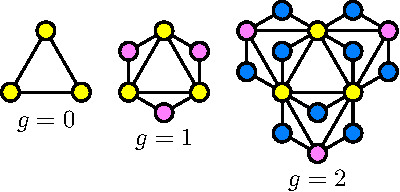
\includegraphics[width=0.75\linewidth]{Pseudofractal-eps-converted-to.pdf}
    \caption{The first several iterations of the pseudofractal scale-free web. }
    \label{psfw1}
\end{figure}
%%%%%%%%%%%%%%%%%%%%%%%%%%%%%%%%%%%%%%%%%%%%%%%%%%%%%%%%%%

\textbf{Kemeny Constant of  Koch Network.}
The Koch network is also built in an iterative way~\cite{ZhZhXiLiGu09}. Let \(\mathcal{M}_{g}\) (\(g \geq 0\)) denote the Koch network after \(g\) iterations. Initially (\(g=0\)), \(\mathcal{M}_{0}\) is a triangle with three
vertices and three edges. For \(g\geq 1\), \(\mathcal{M}_{g}\) is obtained from \(\mathcal{M}_{g-1}\) by
performing the following operations. For each of the three vertices in
every existing triangle in \(\mathcal{M}_{g-1}\), two new vertices are created, both of which and their
``mother'' vertices are connected to one another forming a new triangle. \figref{network} illustrates the growth process of the Koch network.  In network \(\mathcal{M}_{g}\), the number of vertices is \(2\times 4^{g}+1\), and the number of
edges is \(3\times 4^{g}\).  In~\cite{XiLiZh15}, the Kemeny constant \(K(\mathcal{M}_g)\) for \(\mathcal{M}_g\) was obtained to be
\begin{equation}\label{Kg02}
    K(\mathcal{M}_g)=(1+2g)\times 4^g+\frac{1}{3}\,. %\notag
\end{equation}

%%%%%%%%%%%%%%%%%%%%%%%%%%%%%%%%%%%%%%%%%%%%%%%%%%%%%%%%%
% Figure 2
%%%%%%%%%%%%%%%%%%%%%%%%%%%%%%%%%%%%%%%%%%%%%%%%%%%%%
\begin{figure}[!t]
    \centering
    % \includegraphics[width=0.85\linewidth,trim=0 0 0 0]{Koch.eps}
    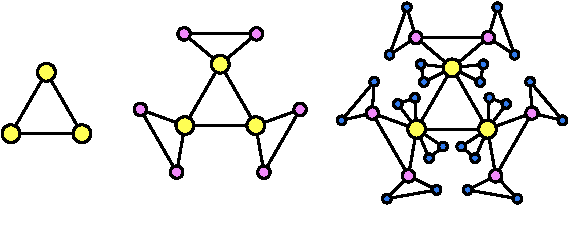
\includegraphics[width=0.85\linewidth]{Koch-eps-converted-to.pdf}
    \caption{Construction process for the Koch network.}
    \label{network}
\end{figure}
%%%%%%%%%%%%%%%%%%%%%%%%%%%%%%%%%%%%%%%%%%%%%%%%%%%%%

\textbf{Kemeny Constant of Cayley Tree.}
Let \(\mathcal{C}_{b,g}(b\ge3,g\ge0)\) represent the Cayley tree after
\(g\) iterations, which are constructed  as follows~\cite{CaCh97,ChCa99}. Initially \((g = 0)\), \(\mathcal{C}_{b,0}\) only contains a central vertex. To obtain \(\mathcal{C}_{b,1}\), we generate  \(b\) vertices and linked them to
the central one. For any \(g>1\), \(\mathcal{C}_{b,g}\) is obtained from \(\mathcal{C}_{b,g-1}\) by performing the following operation. For every periphery vertex of \(\mathcal{C}_{b,g-1}\), \(b-1\) vertices are created and connected to
the periphery vertex. \figref{Cayley} illustrates a special Cayley tree,
\(\mathcal{C}_{3,5}\). In the tree \(\mathcal{C}_{b,g}\), there are \((b(b-1)^g-2)/(b-2)\) vertices and \((b(b-1)^g-2)/(b-2)-1\) edges. In~\cite{JuWuZh13}, the authors  considered a particular Cayley tree \(\mathcal{C}_{3,g}\) corresponding to \(b=3\) and obtained an exact expression for its  Kemeny constant \(K(\mathcal{C}_{3,g})\):
\begin{equation}\label{Kg03}
    K(\mathcal{C}_{3,g})=\frac{3g\times 4^{g+1}-13\times 2^{2g+1} + 35\times 2^g - 9}{2(2^g-1)}.
\end{equation}

%%%%%%%%%%%%%%%%%%%%%%%%%%%%%%%%%%%%%%%%%%%%%%%%%%%%%%%%%
% Figure 3
%%%%%%%%%%%%%%%%%%%%%%%%%%%%%%%%%%%%%%%%%%%%%%%%%%%%%
\begin{figure}[!t]
    \centering
    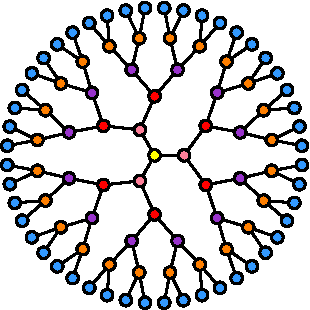
\includegraphics[width=0.6\linewidth,trim=0 0 0 0]{Cayley.pdf}
    %\includegraphics[width=0.5\textwidth]{Labelling.eps}
    \caption{The Cayley tree \(\mathcal{C}_{3,5}\).}
    \label{Cayley}
\end{figure}
%%%%%%%%%%%%%%%%%%%%%%%%%%%%%%%%%%%%%%%%%%%%%%%%%%%%%


\textbf{Kemeny Constant of Extended Tower of Hanoi graph.}  As the name suggests, the extended Tower of Hanoi graph is constructed  based on the Tower of Hanoi graph.  Let \(\mathcal{H}_{g}\)  be the  Tower of Hanoi graph of generation \(g\)~\cite{HiKlMiPeSt13}. The vertex set of \(\mathcal{H}_{g}\) consists of all \(3\)-tuples of integers \(1,2,3\), i.e., \(V(\mathcal{H}_{g})=\{1,2,3\}^g\). All vertices in \(\mathcal{H}_{g}\) are labelled as \((x_1,x_2,\cdots,x_g)\), hereafter written in regular expression form \(x_1x_2\cdots x_g\), with \(x_i\in\{1,2,3\}\) for \(i=1,2,...,g\). Two vertices \(u=u_1u_2\cdots u_g\) and \(v=v_1v_2\cdots v_g\) in \(\mathcal{H}_{g}\) are directly connected by an edge if and only if there exists an \(h(1\le h\le g)\) such that
\begin{enumerate}
    \item \(u_t=v_t\) for \(1\le t\le h-1\);
    \item \(u_h\neq v_h\);
    \item \(u_t=v_h\) and \(v_t=u_h\) for \(h+1\le t\le g\).
\end{enumerate}

Figure~\ref{Sierpinski} illustrates the  Tower of Hanoi graph \(\mathcal{H}_{3}\) and its vertex labeling. In \(\mathcal{H}_{g}\), a vertex having label form \((ii\cdots i)(1\le i\le 3)\) is called an extreme vertex.

%%%%%%%%%%%%%%%%%%%%%%%%%%%%%%%%%%%%%%%%%%%%%%%%%%%%%%%%%
% Figure 4
%%%%%%%%%%%%%%%%%%%%%%%%%%%%%%%%%%%%%%%%%%%%%%%%%%%%%

\begin{figure}[!t]
    \centering
    \subfigure[\(\mathcal{H}_{3}\)]{
        \begin{minipage}[t]{0.5\linewidth}
            \centering
            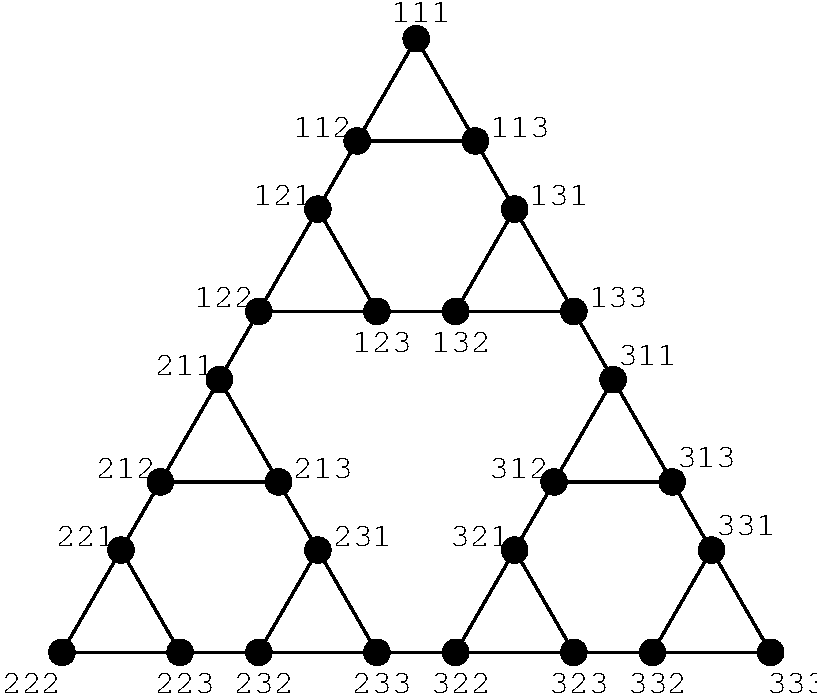
\includegraphics[width=0.95\linewidth,trim=0 0 0 0]{spsk.pdf}
            %\caption{The Sierpi\'nski graph \(\calS_{3,3}\) and its vertex labeling.}
            \label{Sierpinski}
        \end{minipage}%
    }%
    \subfigure[\(\overline{\mathcal{H}}_{3}\)]{
        \begin{minipage}[t]{0.5\linewidth}
            \centering
            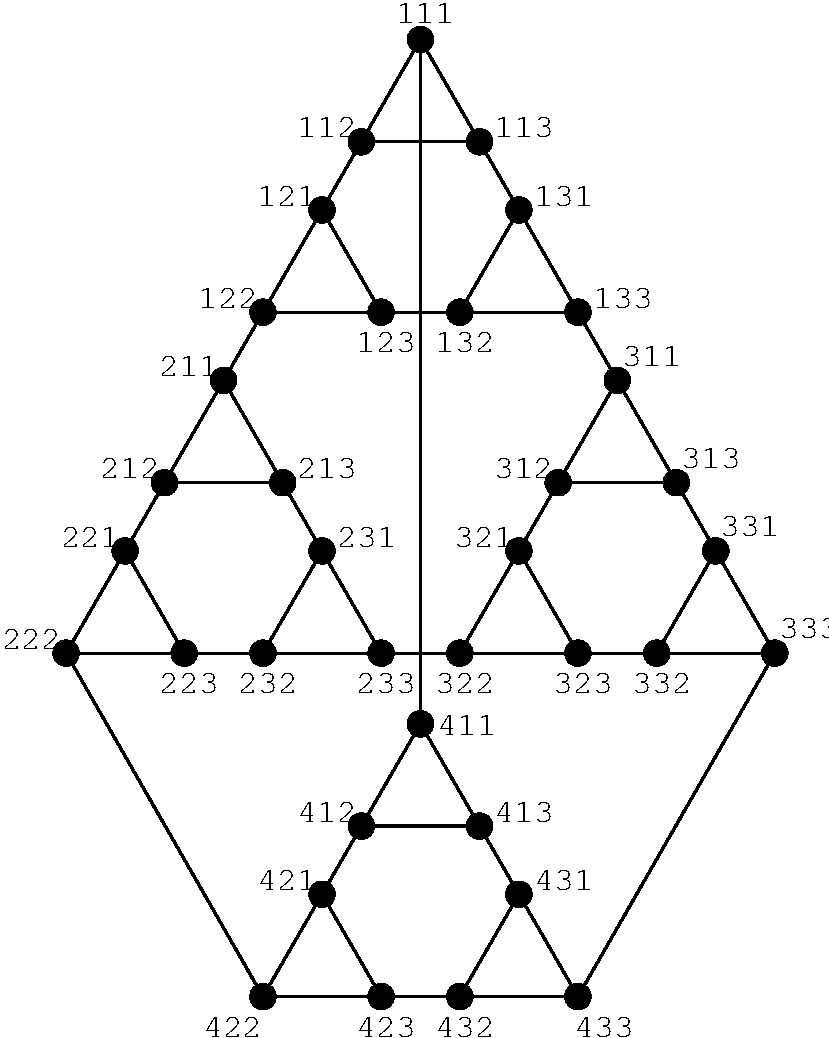
\includegraphics[width=0.95\linewidth,trim=0 0 0 0]{spsklk.pdf}
            %\caption{The extended Sierpi\'nski graph \(\calS^{++}_{3,3}\) and its vertex labeling.}
            \label{exSierpinski}
        \end{minipage}%
    }%
    \centering
    \caption{Illustrations of the Tower of Hanoi graph \(\mathcal{H}_{3}\) and its extension \(\overline{\mathcal{H}}_{3}\), as well as  their vertex labeling.}
\end{figure}
%%%%%%%%%%%%%%%%%%%%%%%%%%%%%%%%%%%%%%%%%%%%%%%%%%%%%

The extended  Tower of Hanoi graph denoted by \(\overline{\mathcal{H}}_{g}(g\ge 1)\)  proposed by Klava\u zar and Mohar~\cite{KlMo05,ZhWuLiCo16,QiDoZhZh20}, is defined as follows. For \(g=1\), \(\overline{\mathcal{H}}_{1}\) is a triangle. For \(g\ge2\),  \(\overline{\mathcal{H}}_{g}\) was obtained from the disjoint union of \(4\) copies of \(\mathcal{H}_{g-1}\), where the extreme vertices in different  replicas of \(\mathcal{H}_{g-1}\) are connected as the 4-vertex complete graph. Figure~\ref{exSierpinski} shows the extended  Tower of Hanoi graph \(\overline{\mathcal{H}}_{3}\) and the its labeling. In graph \(\overline{\mathcal{H}}_{g}\), the number of nodes is \(4\cdot3^{g-1}\), and the number of edges is \(4\cdot3^g/2\). As shown in~\cite{QiZh18}, the Kemeny constant \(K(\overline{\mathcal{H}}_{g})\) for \(\overline{\mathcal{H}}_{g}\) is
\begin{align}
    K(\overline{\mathcal{H}}_{g}) = \frac{32\times5^g\times3^{g-1}-64\times3^{2g-2}-2\times3^g}{10(3^g+3^{g-1}-1)}.
    \label{Kg04}
\end{align}

\textbf{Numerical Results.} We use our algorithm \textsc{ApproxHK} to compute the Kemeny constant on   pseudofractal scale-free web \(\mathcal{F}_{12}\),  Koch network \(\mathcal{M}_{10}\),   Cayley tree \(\mathcal{C}_{3,19}\), and   extended  Tower of Hanoi graph \(\overline{\mathcal{H}}_{13}\). The numerical results are reported in  Table~\ref{tab:Kemeny}, which shows that the approximation algorithm \textsc{ApproxHK} works effectively for the four networks. This again demonstrates the advantage of our proposed algorithm  \textsc{ApproxHK} for large networks.

\begin{table*}[htbp]
    %\tabcolsep=5pt
    \centering
    % \normalsize
    %\fontsize{6.51}{8.0}\selectfont
    \begin{threeparttable}
        \caption{Exact Kemeny constant \(K\),   their approximation \(\tilde{K}\),  relative error \(\rho=\abs{K-\tilde{K}}/K\), and running time (seconds, \(s\)) for \(\tilde{K}\) on networks \(\mathcal{F}_{12}\), \(\mathcal{M}_{10}\), \(\mathcal{C}_{3,19}\) and \(\overline{\mathcal{H}}_{13}\).  \(K\) is obtained via~\eqref{Kg01} and~\eqref{Kg02}, while \(\tilde{K}\) is obtained through algorithm \textsc{ApproxHK} with \(\epsilon=0.2\).}
        \label{tab:Kemeny}
        \begin{tabular}{ccccccc}
            \toprule
            Network                         & Vertices  & Edges     & \(K\)       & \(\tilde{K}\) & Error \(\rho\) & Time\cr
            \midrule
            \specialrule{0em}{3pt}{3pt}
            \(\mathcal{F}_{12}\)            & 797,163   & 1,594,323 & 1,321,776   & 1,322,243     & 0.00035        & 16.71\cr
            \specialrule{0em}{3pt}{3pt}
            \(\mathcal{M}_{10}\)            & 2,097,153 & 3,145,728 & 22,020,096  & 22,015,912    & 0.00004        & 45.70\cr
            \specialrule{0em}{3pt}{3pt}
            \(\mathcal{C}_{3,19}\)          & 1,572,862 & 1,572,861 & 52,953,206  & 52,564,893    & 0.00733        & 31.48\cr
            \specialrule{0em}{3pt}{3pt}
            \(\overline{\mathcal{H}}_{13}\) & 2,125,764 & 3,188,646 & 975,712,653 & 970,030,470   & 0.00582        & 1028\cr
            \specialrule{0em}{3pt}{3pt}
            \bottomrule
        \end{tabular}
    \end{threeparttable}
\end{table*}



\subsection{Performance for Algorithms \textsc{DeterMinGWC} and \textsc{ApproxMinGWC}}


\textbf{Accuracy of Algorithms \textsc{DeterMinGWC} and \textsc{ApproxMinGWC}.} We first demonstrate the accuracy of our algorithms \textsc{DeterMinGWC} and \textsc{ApproxMinGWC} by comparing their results of with the optimum and random solutions on four small-scale networks~\cite{Ku13}: \(\mathit{Zebra}\) with 23 vertices and *** edges, \(\mathit{Zachary\ karate\ club}\) with 34 vertices and *** edges, \(\mathit{Contiguous\ USA}\) with 49 vertices and *** edges, and \(\mathit{Les\ Miserables}\) with 77 vertices and *** edges. For each network, a random solution is obtained by choosing $k$ vertices uniformly at random. Moreover, since these small networks, we are able to compute the optimum solutions by brute-force search. For each $k=1,2,\ldots,5$, we find $k$ vertices  by optimal and stochastic schemes, and \textsc{DeterMinGWC} and \textsc{ApproxMinGWC}, with the error parameter $\epsilon$ in \textsc{ApproxMinGWC} being  \(0.2\). We report the GWC results on these four strategies in~\figref{pic:compare-effect-optimum}. As shown in~\figref{pic:compare-effect-optimum},  the solutions provided by our algorithms \textsc{DeterMinGWC} and \textsc{ApproxMinGWC} are almost identical, with both being very close to the optimum solutions. This indicates that the practical approximation ratios of our algorithms are much better than their theoretical guarantees. In addition,  \textsc{DeterMinGWC} and \textsc{ApproxMinGWC} are far better than the random strategy.



\begin{figure}[!t]
    \centering
    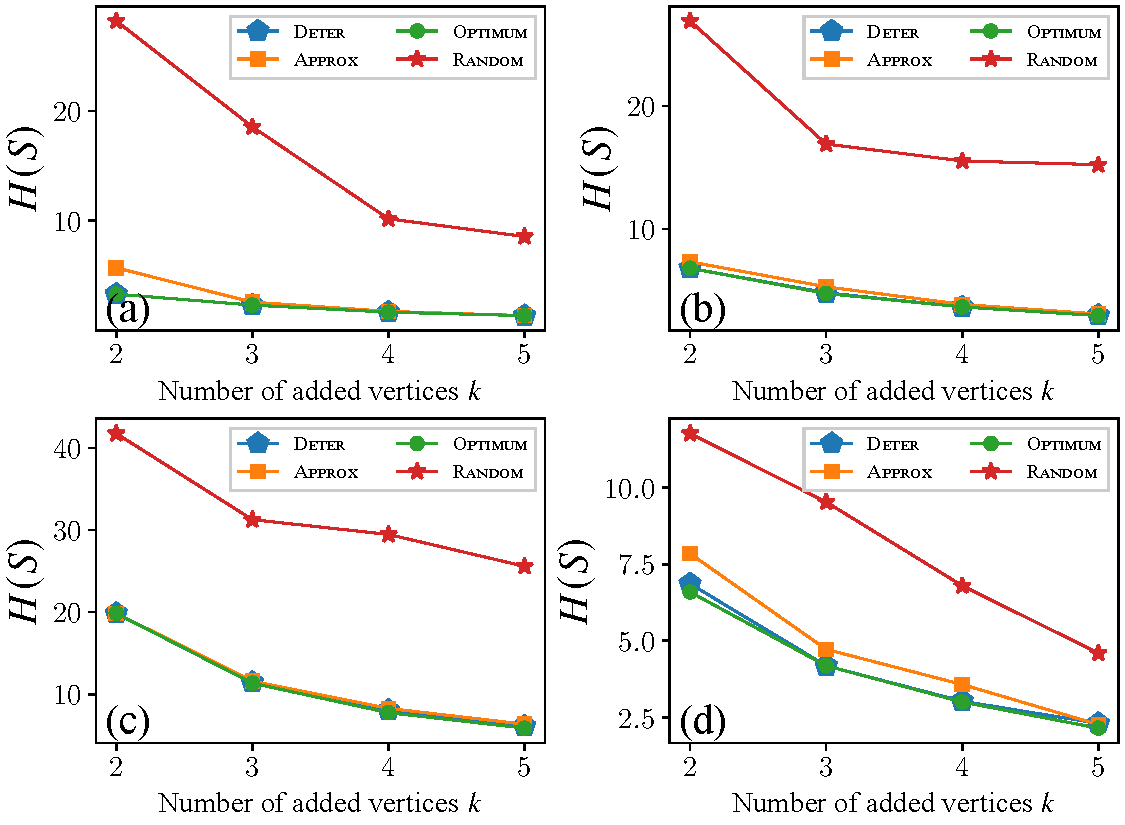
\includegraphics[width=\linewidth]{compare_effects_optimum.pdf}
    \caption{GWC \(\manc{S}\) of vertex group \(S\) computed by four different algorithms(\textsc{DeterMinGWC},\textsc{ApproxMinGWC}, \textsc{Random} and \textsc{Optimum}) on four networks: Zebra (a), Zachary karate club (b), Contiguous USA (c) and Les Miserables (d), where \textsc{DeterMinGWC} and \textsc{ApproxMinGWC} are denoted as \textsc{Deter} and \textsc{Approx} in the legend to save space.\label{pic:compare-effect-optimum}}
\end{figure}

We continue to demonstrate the effective of our algorithms \textsc{DeterMinGWC} and \textsc{ApproxMinGWC} by comparing their performance  with three baseline algorithms: \text{Top-Absorb}, \text{Top-Degree}, and \text{Top-PageRank}. \text{Top-Absorb} simply selects \(k\) vertices with the lowest value of walk centrality, \text{Top-Degree} selects \(k\) vertices with the largest degrees, while \text{Top-PageRank} selects \(k\) vertices with the largest  PageRank values. We execute these five strategies of vertex selection on eight medium-sized networks, with the parameter $\epsilon$ in \textsc{ApproxMinGWC} being  \(0.2\). The results for these schemes are shown in \figref{pic:compare-effect1} and \figref{pic:compare-effect2}. As displayed in these two figures, both of our algorithms produce similar approximate solutions, outperforming the other three baseline strategies.

\begin{figure}[!t]
    \centering
    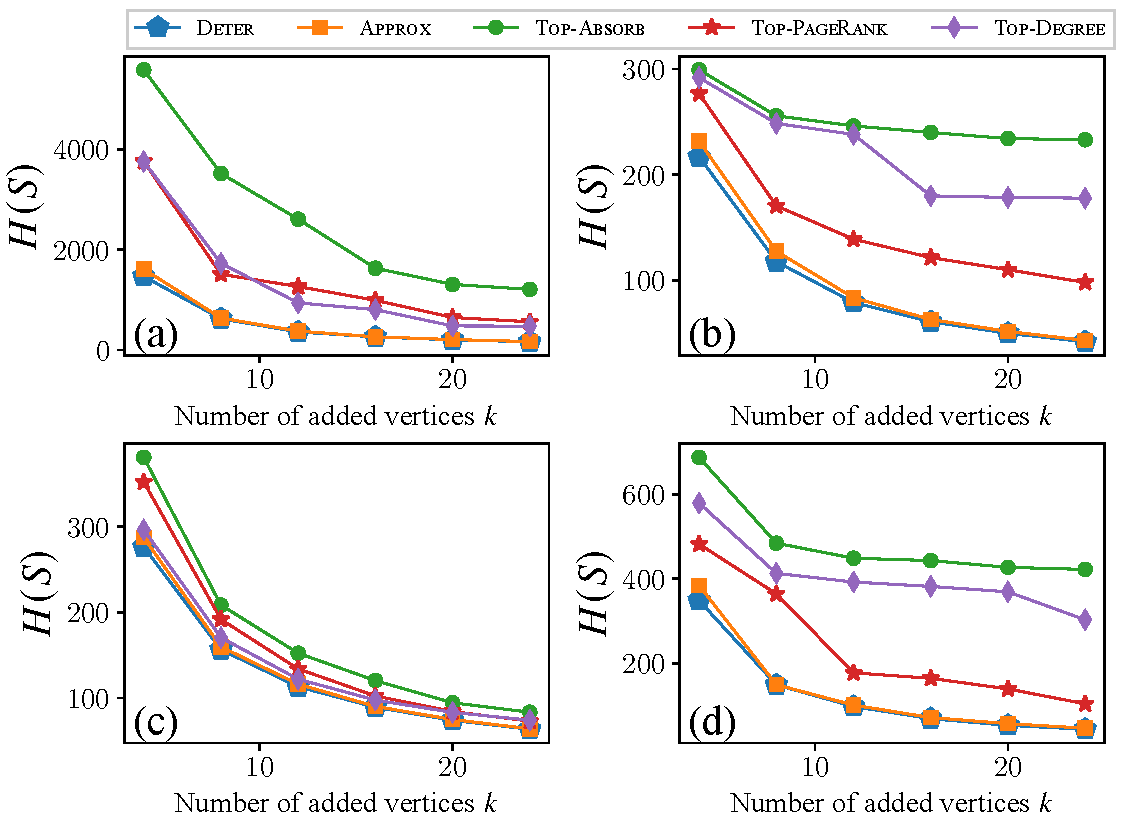
\includegraphics[width=\linewidth]{compare_effects_exact1.pdf}
    \caption{GWC \(\manc{S}\) of vertex group \(S\) computed by four different algorithms(\textsc{DeterMinGWC},\textsc{ApproxMinGWC},\text{Top-Absorb} and \text{Top-Degree}) on four networks: CA-GrQc (a), ego-Facebook (b), Euroroads (c) and US power grid (d), where \textsc{DeterMinGWC} and \textsc{ApproxMinGWC} are denoted as \textsc{Deter} and \textsc{Approx} in the legend to save space.\label{pic:compare-effect1}}
\end{figure}

\begin{figure}[!t]
    \centering
    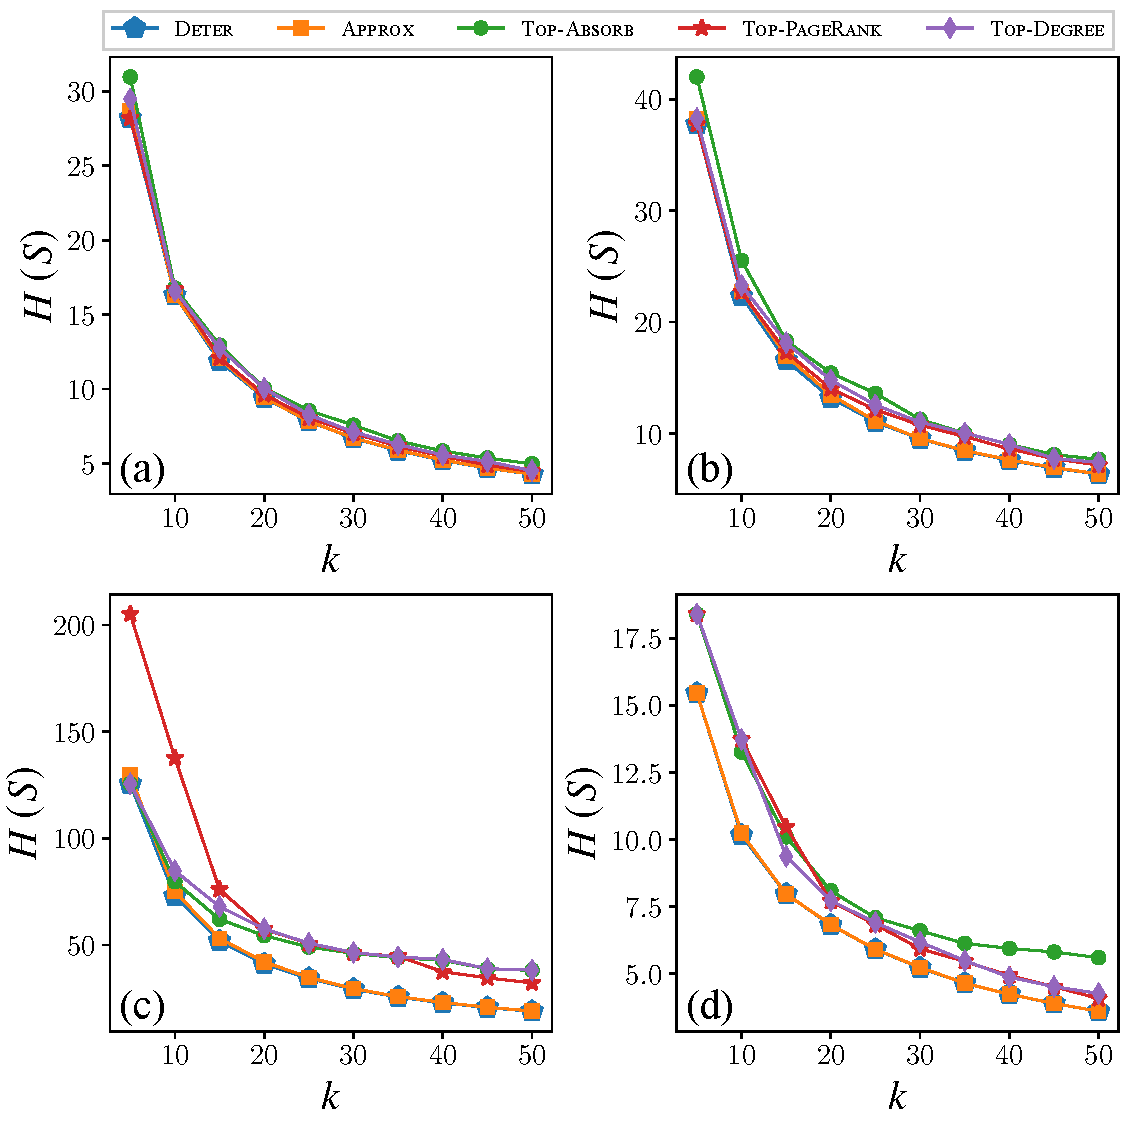
\includegraphics[width=\linewidth]{compare_effects_exact2.pdf}
    \caption{GWC \(\manc{S}\) of vertex group \(S\) computed by four different algorithms \textsc{DeterMinGWC},\textsc{ApproxMinGWC},\text{Top-Absorb} and \text{Top-Degree} on four networks: Hamster friends (a), Hamster full (b), Reactome (c) and Route views (d), where \textsc{DeterMinGWC} and \textsc{ApproxMinGWC} are denoted as \textsc{Deter} and \textsc{Approx} in the legend to save space.\label{pic:compare-effect2}}
\end{figure}

\textbf{Comparison of Efficiency between \textsc{DeterMinGWC} and \textsc{ApproxMinGWC}.} Although both \textsc{DeterMinGWC} and \textsc{ApproxMinGWC} are very effective, below we demonstrate that \textsc{ApproxMinGWC} is significantly more efficient than \textsc{DeterMinGWC}, particularly in large networks. To this end, we compare the running time of \textsc{DeterMinGWC} and \textsc{ApproxMinGWC} and the GWC of vertex group returned by these two algorithms on a set of real-life networks. For each network, we use \textsc{DeterMinGWC} and \textsc{ApproxMinGWC} to select \(k=10\) vertices. We present the results in \tabref{tab:running-time}, from which we observe that the running time of  \textsc{ApproxMinGWC} is much lower than  that of \textsc{DeterMinGWC}, while the vertex sets returned by  \textsc{DeterMinGWC} and \textsc{ApproxMinGWC} have almost the same GWC.

The efficiency advantage of   \textsc{ApproxMinGWC} over  \textsc{DeterMinGWC} becomes more obvious for larger networks. \tabref{tab:running-time} shows the difference of running time between   \textsc{DeterMinGWC} and \textsc{ApproxMinGWC} increases rapidly when the networks become larger. For those networks marked with \(\ast\) in \tabref{tab:running-time},  \textsc{DeterMinGWC} cannot run due to the memory and time limitations, while  \textsc{ApproxMinGWC} still works well. In particular, \textsc{ApproxMinGWC} scales to massive networks with one million nodes. For example, for the roadNet-CA network with almost two million nodes, \textsc{ApproxMinGWC} solves the MinGWC problem in about four hours. Thus, \textsc{ApproxMinGWC} is both efficient and effective, and scalable to massive networks.

\iffalse
    \textbf{Comparison of Efficiency between \textsc{DeterMinGWC} and \textsc{ApproxMinGWC}.}
    Finally, we demonstrate that the \textsc{ApproxMinGWC} is significantly more efficient than the \textsc{DeterMinGWC} algorithm, particularly when applied to large networks.
    We test both algorithms on a wider range of real networks.
    For each network, we use \textsc{DeterMinGWC} and \textsc{ApproxMinGWC} separately to solve the GWC minimization problem, with \(k=10\) and \(\epsilon=0.2\).
    The running times of both algorithms are shown in \tabref{tab:running-time}.

    From \tabref{tab:running-time}, we can observe that the running time of \textsc{ApproxMinGWC} is proportional to the number of edges in the network, leading to an increase in the speedup ratio of \textsc{ApproxMinGWC} as the network size grows.
    Furthermore, \tabref{tab:running-time} indicates that when processing networks marked with \(\ast\),
    \textsc{ApproxMinGWC} remains usable while \textsc{DeterMinGWC} fails due to its high time complexity.
    This result demonstrates the scalability of \textsc{ApproxMinGWC} when applied to large networks.
\fi


\begin{table}[htbp]
    \tabcolsep=8pt
    \centering
    \fontsize{8.0}{8.8}\selectfont
    \begin{threeparttable}
        \caption{The running time (seconds, \(s\)) of \textsc{DeterMinGWC} and \textsc{ApproxMinGWC} (denoted as \textsc{Deter} and \textsc{Approx} in the table to save space) with various \(\epsilon\) on several realistic networks}
        \label{tab:running-time}
        \begin{tabularx}{8.25cm}{c p{1cm} p{0.5cm} p{0.5cm} p{0.5cm}}
            \toprule[1pt]
            \multirow{2}{*}{Network}        &
            \multirow{2}{*}{\textsc{Deter}} &
            \multicolumn{3}{c}{\textsc{Approx} (\(s\)) for various \(\epsilon\)}\cr
            \cmidrule{3-5}
                                            & (\(s\)) & \(0.3\) & \(0.25\) & \(0.2\)\cr
            \midrule
            Jazz musicians                  & 0.214   & 0.157   & 0.178    & 0.194\cr
            Euroroads                       & 0.498   & 0.239   & 0.277    & 0.281\cr
            Hamster friends                 & 1.183   & 0.348   & 0.450    & 0.629\cr
            Hamster full                    & 1.267   & 0.402   & 0.525    & 1.049\cr
            Facebook (NIPS)                 & 10.20   & 1.956   & 2.919    & 4.349\cr
            CA-GrQc                         & 10.74   & 0.686   & 0.896    & 0.968\cr
            US power grid                   & 17.62   & 0.500   & 0.634    & 0.977\cr
            Reactome                        & 30.13   & 3.593   & 4.680    & 7.329\cr
            Route views                     & 37.55   & 0.582   & 0.704    & 1.024\cr
            CA-HepTh                        & 85.83   & 1.108   & 1.602    & 2.476\cr
            Sister cities                   & 143.3   & 3.246   & 3.974    & 7.013\cr
            Pretty Good Privacy             & 157.7   & 3.844   & 5.170    & 7.657\cr
            CA-HepPh                        & 180.8   & 6.601   & 9.775    & 15.74\cr
            Astro-ph                        & 715.8   & 13.51   & 18.26    & 31.31\cr
            CAIDA                           & 2272    & 6.355   & 7.838    & 11.28\cr
            Brightkite*                     & --      & 23.31   & 32.68    & 54.21\cr
            Livemocha*                      & --      & 177.0   & 250.6    & 392.1\cr
            WordNet*                        & --      & 83.89   & 124.5    & 221.4\cr
            Gowalla*                        & --      & 129.1   & 195.7    & 342.8\cr
            com-DBLP*                       & --      & 232.7   & 399.1    & 756.8\cr
            Amazon*                         & --      & 349.5   & 652.3    & 1082\cr
            roadNet-PA*                     & --      & 2215    & 3349     & 5714\cr
            YouTube*                        & --      & 1482    & 2197     & 3661\cr
            roadNet-TX*                     & --      & 3135    & 4464     & 9338\cr
            roadNet-CA*                     & --      & 5445    & 8214     & 14458\cr
            \bottomrule
        \end{tabularx}
    \end{threeparttable}
\end{table}

\section{Related Works}

Many researchers have noticed the connection between random detour time and their proposed centralities.
Ranjan et al.~\cite{RaZh13} presented \textit{topological centrality} \(\cscr^*(u)\) as the reciprocal of \(\lap^\dagger_{[u,u]}\), and found that \(\cscr^*(u)\) can be represented by random detour time and hitting time, that is, \({\cscr^*(u)}^{-1}\propto \sum_{i=1}^n\sum_{j=1}^n\mypar{D_{ij}(u)-H_{ij}}\).
Gangemi et al.~\cite{GaLePaGoLiZh15} simply took variants of random detour time as components of \textit{pivotality}, which is the measure of node reachability.
We prove that random detour time is also related to Kemeny constant and absorbing random-walk centrality.
This connection also holds for the case of multiple nodes.

There also exist various random walk-based centralities, such as the \textit{Random Walk Decay Centrality}~\cite{WaRaSk19} and the \textit{Group-to-group random walk betweenness centrality}~\cite{GiBaRa21}, both of them are variants of existing centralities.
Besides, Mavroforakis et al.~\cite{MaMaGi15} presented \textit{\(k\) absorbing random-walk centrality}, which is the most directly related to our work.
We give new proofs on the monotonicity and supermodularity of GWC from the perspective of numerical analysis, which is more concise and intuitive.
Moreover, we design and implement a nearly linear algorithm for GWC minimization problem, which is proved to have an approximation guarantee.

Admittedly, many existing studies have focused on the notion of selecting \(k\) nodes in the network to optimize some quantities related to absorbing random walk, such as absorbing distance~\cite{LiYuHuCh14,MoBaZhPe20} and absorbing probability~\cite{RoGl16}.
However, computing these quantities on infinite random walk models requires time-consuming matrix inversions.
Most of researchers use finite random walk models to approximate the infinite case, except for Rosenfeld et al.~\cite{RoGl16}, who use LU decomposition to reduce the complexity of computing absorbing probability.
Instead of constructing finite random walk models, our work focus on the infinite random walk model, use a nearly linear algorithm to minimize GWC, which has a \(1-\frac{k}{k-1}\cdot\frac{1}{e}-\epsilon\) approximate factor for any error parameter \(\epsilon\in(0,1)\).

\section{Conclusions}

The hitting time of random walks arises in many practical scenarios.
However, exactly computing the hitting time is prohibitively expensive, making it difficult to solve corresponding optimization problems.
In this paper, we studied absorbing random-walk centrality and Kemeny constant of a graph, both of which are actually weighted average of hitting times and have found wide applications.
We established a link between the two quantities and reformulated them in terms of quadratic forms of the pseudoinverse of graph Laplacian.
Subsequently, we extended the notion of mean hitting time to multiple vertices, proposing Group Walk Centrality (GWC) and its minimization problem.
We demonstrated the monotonicity and supermodularity of this newly proposed centrality, expressing it in terms of the inverse of a SDDM matrix.
Moreover, we provided a randomized approximation algorithm with probabilistic guarantee, which computes the walk centrality for all vertices and Kemeny constant in nearly linear time with respect to the number of edges.
Based on this algorithm, we provided another nearly linear greedy approximate algorithm to solve the minimization problem of GWC, which is proved to be NP-hard.
Finally, we conducted extensive experiments on various real-world and model networks, which show that the proposed algorithms are both efficient and accurate, especially for large-scale networks.

\bibliographystyle{IEEEtran}
\balance
\bibliography{refs}
% \begin{IEEEbiography}[\biophoto{xhs.jpg}]{Haisong Xia}
\begin{IEEEbiographynophoto}{Haisong Xia}
    received the B.S. degree in computer science from Fudan University, Shanghai, China, in 2022. He is currently pursuing the master's degree in the School of Computer Science at Fudan University.
    His current research interests include network science, spectral graph theory and social network analysis.
\end{IEEEbiographynophoto}

% \begin{IEEEbiography}{Wanyue Xu}
\begin{IEEEbiographynophoto}{Wanyue Xu}
    (Student Member, IEEE) received the B.Eng. degree in computer science and technology from Shangdong University, Weihai, China, in 2019. She is currently pursuing the master's degree with the School of Computer Science, Fudan University, Shanghai, China.
    Her research interests include network science, graph data mining, social network analysis, and random walks.
\end{IEEEbiographynophoto}

% \begin{IEEEbiography}{Zuobai Zhang}
\begin{IEEEbiographynophoto}{Zuobai Zhang}
    received the B.S. degree  in computer science from Fudan University, Shanghai, China, in 2021. 	He is currently pursuing the Ph.D. degree at Mila - Qu\'{e}bec AI Institute, Canada. His research interests include graph algorithms, graph representation learning, and drug discovery.
\end{IEEEbiographynophoto}

% \begin{IEEEbiography}{Zhuoqing Song}
\begin{IEEEbiographynophoto}{Zhuoqing Song}
    received the B.S. degree in mathematics and applied mathematics in 2019 from Fudan University, Shanghai, China, where he is currently working toward the Ph.D. degree in applied mathematics. His research interests include decentralized optimization, graph algorithms, and machine learning.
\end{IEEEbiographynophoto}

% \begin{IEEEbiography}[\biophoto{zzz.jpg}]{Zhongzhi Zhang}
\begin{IEEEbiographynophoto}{Zhongzhi Zhang}
    (Member, IEEE) received the B.Sc. degree in applied mathematics from Anhui University, Hefei, China, in 1997 and the Ph.D. degree in management science and engineering from Dalian University of Technology, Dalian, China, in 2006. \\
    From 2006 to 2008, he was a Post-Doctoral Research Fellow with Fudan University, Shanghai, China, where he is currently a Full Professor with the School of Computer Science. He has published over 150 papers in international journals or conferences. He has over 3300 ISI Web of Science citations with an H-index of 33 according to the Clarivate. He was selected as one of the most cited Chinese researchers
    (Elsevier) in 2019 and 2020. His current research interests include network science, graph data mining, social network analysis, spectral graph theory, and random walks. \\
    Dr. Zhang was a recipient of the Excellent Doctoral Dissertation Award of Liaoning Province, China, in 2007, the Excellent Post-Doctor Award of Fudan University in 2008, the Shanghai Natural Science Award (third class) in 2013, and the Wilkes Award for the best paper published in The Computer Journal in 2019. He is a member of the IEEE.
\end{IEEEbiographynophoto}

\end{document}
